\ifdefined\pdfminorversion\pdfminorversion=7\fi
\documentclass[11pt]{article}

\usepackage[letterpaper,margin=0.78in]{geometry}
\usepackage[T1]{fontenc}
\usepackage[utf8]{inputenc}
\usepackage{mathptmx}
\usepackage{microtype}
\usepackage{amsmath,amssymb,bm,amsthm}
\usepackage{booktabs,array,graphicx,subcaption}
\captionsetup{font=small}
\usepackage[numbers,sort&compress]{natbib}
\usepackage{xcolor}
\usepackage{lineno}
\usepackage[hidelinks,hypertexnames=false]{hyperref}

\ifdefined\DendriticLocalLearningRepoRoot
  \graphicspath{{journal/figures/}}
  \newcommand{\journalbibliography}{journal/references}
\else
  \graphicspath{{figures/}}
  \newcommand{\journalbibliography}{references}
\fi
\raggedbottom
\setlength{\textfloatsep}{10pt plus 2pt minus 2pt}
\setlength{\floatsep}{8pt plus 2pt minus 2pt}
\setcounter{topnumber}{2}
\setcounter{totalnumber}{3}
\renewcommand{\topfraction}{0.95}
\renewcommand{\textfraction}{0.04}
\renewcommand{\floatpagefraction}{0.65}

\newtheorem{theorem}{Theorem}
\newtheorem{proposition}{Proposition}
\newcommand{\E}{\mathbb{E}}
\newcommand{\R}{R^{\mathrm{tot}}}
\DeclareMathOperator{\tr}{tr}

\title{Dendritic morphology as a dictionary for local credit assignment}

\author{Houman Safaai$^{1,*}$, Maceo Richards$^{1}$, and Bernardo L. Sabatini$^{1,2,*}$\\[4pt]
\small $^{1}$Kempner Institute for the Study of Natural and Artificial Intelligence at Harvard University, Cambridge, MA, USA\\
\small $^{2}$Department of Neurobiology, Howard Hughes Medical Institute, Harvard Medical School, Boston, MA, USA\\
\small $^{*}$Correspondence: \texttt{houman\_safaai@harvard.edu}; \texttt{bernardo\_sabatini@hms.harvard.edu}}
\date{}

\begin{document}
\maketitle
\linenumbers

\begin{abstract}
Dendritic trees compartmentalize synaptic inputs, but which spatial distinctions a learning signal must preserve is unclear. We describe delivered credit as combinations of spatial profiles constrained by morphology. In image classifiers with one dendritic neuronal layer, preserving neuronal identity accounts for most of the feedback benefit. Contextual conflict favors branch selection, while hierarchical distractors favor ancestry grouping at a bandwidth predicted by the task. Targets with matched input-sensitivity spectra develop different learned credit spectra and tolerance of fixed profiles; a local inhibitory gate also supports learning of opposing branch tuning in a conductance tree. Serial compartments help when nuisance-factor information is distributed across modules. Reconstructed arbors compress modeled passive perturbation fields through ancestry profiles, and focal shunts regulate their gains with selectivity set by electrotonic state. Measured visual responses provide no evidence of preferential ancestry alignment in the sampled cells. The framework links task structure to useful credit distinctions while separating available delivery patterns from the mechanisms that generate their coefficients.
\end{abstract}

\section*{Introduction}

Learning must link a synapse's local activity to its contribution to a circuit outcome. Cable filtering, nonlinear integration and spatially organized inhibition make locations within a dendritic tree functionally distinct \citep{rall1962dendrites,koch1999biophysics,poirazi2003pyramidal,london2005dendritic,spruston2008pyramidal,branco2010single,larkum2013cellular}. These differences expand computation, but when does branching also help distribute useful learning signals?

Credit assignment asks how changing a synapse would affect task error. Backpropagation (BP) answers this by calculating the loss gradient---the sensitivity of task error to each parameter \citep{rumelhart1986learning}; related sensitivity calculations apply to recurrent and steady-state networks \citep{almeida1987asynchronous,pineda1987recurrent}. For a point neuron, each incoming-weight gradient is the product of a locally available sensitivity, called eligibility, and a neuron-specific learning signal. Hebbian plasticity captures the association between local pre- and postsynaptic variables \citep{hebb1949organization}, while three-factor rules combine that eligibility with an outcome-dependent signal \citep{fremaux2016threefactor}. Here, a rule is local when a synapse uses its own eligibility and an available learning signal. This definition does not require that the signal itself be computed locally.

Biologically motivated learning theories differ in how they obtain such signals. Feedback alignment communicates errors through separate pathways \citep{lillicrap2016feedback,nokland2016dfa}; equilibrium, predictive and prospective methods infer target states or errors from dynamics \citep{scellier2017equilibrium,whittington2017predictive,song2024prospective}; eligibility propagation combines temporal traces with neuron-specific signals \citep{bellec2020eprop}. One number shared across neurons carries less task information than separately assigned neuronal signals, although each synapse still has its own eligibility \citep{werfel2005learning,whittington2019theories,lillicrap2020backprop}. Recent causal evidence for distinct instructive signals across neuronal populations motivates asking what additional distinctions are useful within a neuron's arbor \citep{francioni2026vectorized}.

We describe this organization using a \emph{route dictionary}: a set of spatial profiles for delivering learning signals. A route identifies the locations reached by a signal; its profile specifies their relative amplitudes, and a coefficient scales that profile on a given trial. Each dictionary column stores one profile. A shared profile broadcasts throughout an arbor, while several profiles can distinguish subtree addresses. Their linear combinations give the available fields. We use \emph{basis} for linearly independent profiles and \emph{dictionary} when profiles may be redundant. Morphology constrains the available routes; the task and teaching mechanism determine useful coefficients.

Conductance changes the gains of anatomical delivery routes. Excitatory and inhibitory contacts open nonnegative conductances whose reversal potentials determine current; inhibition can lower input resistance and attenuate other inputs even when its own current is small \citep{koch1983nonlinear,holt1997shunting,chance2002gain,gidon2012inhibition,lovettbarron2012regulation}. Rescaling a delivery channel preserves its spatial profile, whereas altered cable transport can reshape how local voltage affects somatic output and task error.

Dendritic models already connect nonlinear compartments and structural plasticity to memory capacity \citep{poirazi2001capacity}, and branch-specific plasticity can organize nonlinear feature combinations \citep{legenstein2011branch}. Successive computations in artificial trees and detailed cortical models also establish substantial forward capacity \citep{jones2021successive,beniaguev2021single}. Dendritic learning theories supply mechanisms for somatic prediction, segregated teaching, interneuron-mediated errors, bursts and prospective dynamics \citep{urbanczik2014dendritic,schiess2016somatodendritic,guerguiev2017segregated,sacramento2018dendritic,payeur2021burst,ellenberger2026gle,richards2019dendritic}; cable-learning models optimize reconstructed neurons using synaptic sensitivities \citep{bicknell2021synaptic}. Our question concerns the spatial information these learning mechanisms must preserve across an arbor.

The conductance-tree gradient factorization and LocalCA rule were introduced in our predecessor preprint \citep{safaai2026localcredit}. This Article extends those foundations with controlled task-to-credit comparisons, matched-spectrum and conductance learning experiments, and anatomical transport and response tests.

We compare the value of preserving neuronal identity, branch selection, ancestry grouping and example-dependent credit across interacting branches. Morphology supplies candidate patterns and conductance regulates their expression. We establish forward compatibility before interpreting learning gaps; measured responses test the anatomical proposal. The question is which distinctions useful credit must preserve, rather than whether finer feedback is always better.

\section*{Results}

\subsection*{Exact gradients separate local sensitivity from downstream credit}

A useful synaptic update combines local sensitivity with the effect that the change would have on task error. For a point neuron $y_u=f_u(\sum_iw_ix_i+b_u)$, the chain rule gives $\partial\mathcal L/\partial w_i=x_if'_u\delta_u$, where $x_i$ and $w_i$ are synaptic input and weight, $b_u$ is bias, and $\delta_u=\partial\mathcal L/\partial y_u$ is the neuronal error. The derivative $f'_u$ is evaluated at the current input sum. Thus local eligibility $x_if'_u$ and task-derived credit supply different information (Fig.~\ref{fig:framework}A).

We replace the point neuron by a rooted tree with spatially distinct addresses, with soma \(n=0\), compartment voltage \(V_n\), and nonnegative synaptic conductances \(g_i\). A contact with reversal potential \(E_i^{\mathrm{rev}}\) and nonnegative activity \(x_i\) contributes current \(g_ix_i(E_i^{\mathrm{rev}}-V_n)\). In the directed artificial trees, child outputs drive their parents and a terminal-to-soma pass computes the steady state. Total input resistance \(R_n^{\mathrm{tot}}\) is the reciprocal of the summed leak, excitatory, inhibitory and child-coupling conductances (Methods). Differentiating the current balance yields
\begin{equation}
\frac{\partial\mathcal L}{\partial g_i}
=\underbrace{x_iR_n^{\mathrm{tot}}(E_i^{\mathrm{rev}}-V_n)}_{\mathrm{local\ eligibility}}
\underbrace{\delta^V_{n,u}}_{\partial\mathcal L/\partial V_n}.
\label{eq:factorization}
\end{equation}
Both excitatory (E) and inhibitory (I) contacts obey this factorization (Fig.~\ref{fig:framework}A). Eligibility tells how conductance changes local voltage; compartment credit tells how that voltage changes task loss.

Here voltage error is a loss derivative, not a voltage difference. In a directed tree, each compartment has one path to the soma. Its exact voltage error is
\begin{equation}
\delta^V_{n,u}=\delta^V_{0,u}\widetilde\alpha_n,
\qquad
\widetilde\alpha_n=
\prod_{(i\to k)\in\operatorname{path}(n\to0)}
f_i'(V_i)R_k^{\mathrm{tot}}g_{i\to k}^{\mathrm{den}}.
\label{eq:pathgain}
\end{equation}
Here \(f'_i(V_i)\) is the child compartment's output derivative, \(g_{i\to k}^{\mathrm{den}}\) is its coupling conductance to parent \(k\), and \(\delta^V_{0,u}=f'_0(V_0)\delta_u\) is the somatic voltage error. Thus the path multiplier \(\widetilde\alpha_n\) converts one somatic error into a spatial field. The conductance-only component of this product is attenuated by additional conductance on a path's ancestors; branch nonlinearities and forward voltages can change as well (Supplementary Section~S1).

Reciprocal cables instead require a joint adjoint calculation of how local currents affect task loss (Methods). These mathematical sensitivities do not establish a biological error-transmission mechanism.

Our local credit assignment (LocalCA) rule retains the local sensitivity but supplies an approximate learning signal to each compartment. A hat denotes this delivered field:
\begin{align}
\widehat\nabla_{g_i}\mathcal L
=x_iR_n^{\mathrm{tot}}(E_i^{\mathrm{rev}}-V_n)\widehat\delta^V_{n,u},
\label{eq:dendriticlocalrule}
\\
\widehat{\bm\delta}^{V}_u=A_u\bm c_u.
\label{eq:routedfield}
\end{align}
Columns of \(A_u\in\mathbb R^{N_u\times K}\) are fixed spatial delivery profiles over \(N_u\) routed nonsomatic compartments; \(\bm c_u\) contains their example-dependent coefficients. To distinguish coefficient generation from delivery gain, we can write \(\bm c_u=\Gamma_u\bm c_u^{\rm source}\), where diagonal \(\Gamma_u\) scales each profile and \(\bm c_u^{\rm source}\) is the supplied signal (Fig.~\ref{fig:framework}A). Broadcast, subtree and compartment profiles give increasingly detailed spatial addresses (Fig.~\ref{fig:framework}B). This linear delivery model does not follow automatically from the forward cable equations and does not specify how a circuit estimates the coefficients.


At \(K=1\), the all-ones column \(A_u=\bm1\) broadcasts one coefficient through the arbor; at \(K=N_u\), the identity matrix \(A_u=I\) can reproduce the full nonsomatic field. Nested subtrees provide intermediate dictionaries. Profile count, rank (the number of independent profiles) and coefficient information are distinct resources. Exact path transport combines one somatic scalar with state-dependent local derivatives; it does not require an independent external error for every compartment.

Capture is the fraction of squared learning-signal magnitude that a dictionary can reproduce. For a nonzero field \(\bm\delta\),
\[
\mathcal C(A;\bm\delta)=\frac{\|P_A\bm\delta\|^2}{\|\bm\delta\|^2},
\qquad P_A=AA^\dagger.
\]
Here \(P_A\) gives the best least-squares reconstruction from the profiles; \(A^\dagger\) is the Moore--Penrose pseudoinverse and \(\|\cdot\|\) the Euclidean norm. Thus capture is a fraction of squared field magnitude, not a fraction of correct decisions. The mean of these per-field ratios weights fields equally. In contrast, \(\tr(P_AC)/\tr(C)\), with \(C=\mathbb E[\bm\delta\bm\delta^{\mathsf T}]\), is the fraction of total ensemble energy captured, weighting fields by their energy. Here \(C\) is the uncentered second-moment matrix and \(\tr\) denotes its trace, the sum of diagonal entries. The two capture measures need not agree. Projection chooses the best coefficients in the specified metric; an implemented learning rule need not supply them.

The expansion applies in a specified coordinate. In the nonlinear image models, we route errors of compartment outputs and retain the local output derivative in eligibility; voltage-error capture is reported separately. Identity-output conductance trees use voltage errors directly. Supplementary Table~S2 compares the coordinates, coefficient sources and state dependence. Dictionary capacity answers what fields can be delivered; learning experiments determine which distinctions improve performance.

A restricted dictionary can also filter noise. In a controlled update-space model, projection removes update variation outside the chosen span. A narrower span that retains most of the useful gradient can give a better one-step guarantee when it admits less noise, despite discarding some signal (Fig.~\ref{fig:framework}C). If the span contains the entire gradient, its mean is preserved. A one-step smoothness bound formalizes this balance between retained descent and update variance (Methods; Supplementary Fig.~S2). Its initialization utility did not select the best final morphology: in a separate 12,800-fit prospective experiment, it lost to a fixed maximum-budget tree in all twenty seed averages in both selection arms (Supplementary Fig.~S33). The local filtering principle motivates testing useful spatial distinctions without assuming that one initial score predicts the outcome of an entire learning trajectory.

\subsection*{One signal per neuron captures most of the image-task learning benefit}

We first tested credit resolution on image classification. All image benchmark networks used one dendritic layer and a trainable linear readout. In the primary comparisons, the readout supplied exact neuronal output errors before the feedback intervention. The MNIST comparison used 128 directed \([3,3]\) trees, each with three proximal and nine terminal compartments, receiving flattened images. Shunting and raw-additive architectures shared the graph, initial contact construction, nonlinearities and training protocol, with architecture-specific initialization. The additive control removed reversal-potential driving forces and the conductance denominator, retaining signed current summation without shunting.

Six rules separated neuronal identity, spatial resolution and learning in the dendritic core (Fig.~\ref{fig:framework}B,D). A strict scalar shared one signal across neurons; neuron-specific feedback broadcast each neuron's own output error through its arbor. A projected one-profile rule averaged the exact activation errors over all twelve nonsomatic compartments, while three subtree profiles averaged them within each proximal compartment and its three children. Both projections acquired coefficients from the same exact field and preserved its common-mode mean at identical parameters, although their field norms could differ. Exact transport retained every compartment error. A decoder-only reference trained the readout while freezing the core. Three development seeds selected each rule's rate from three common multipliers; ten fresh paired seeds per architecture evaluated selected and original common rates over 180 epochs (Methods; Supplementary Fig.~S7A,B).

At selected rates, neuron-specific feedback exceeded the strict scalar by 9.23 percentage points in shunting trees and 7.46 points in additive trees, reaching 97.12\% and 97.11\% accuracy. Decoder-only learning reached 80.96\% and 89.57\%, respectively (Fig.~\ref{fig:framework}D). Increasing the projected dictionary from one to three profiles changed accuracy by only 0.049 points in shunting trees (95\% paired interval, $-0.048$ to 0.141) and 0.036 points in additive trees ($-0.056$ to 0.122; Fig.~\ref{fig:framework}E). The common-rate comparison gave similarly small differences (Supplementary Fig.~S7C). Exact transport added 0.010 points over neuron-specific feedback in shunting trees, but 0.182 points in additive trees (0.114--0.252; positive in all ten seeds). Both exact transport and one projected profile reached about 97.3\% in additive trees. Most learning benefit therefore came from preserving neuronal coordinates; the smaller additive improvement was attainable without separating subtrees.

A separate fifteen-seed cohort and exact-gradient checks showed spatial structure in trained fields (Supplementary Section~S2 and Fig.~S7E--G): moving from one to three profiles raised mean voltage-credit capture from 0.480 to 0.625 in shunting trees and from 0.519 to 0.718 in additive trees. The new checkpoint analysis likewise found improved capture without a corresponding accuracy gain from subtree distinctions (Supplementary Fig.~S7D). It reports activation-space capture, matching the trained projections, with voltage-space results supplied separately. These reconstructions measure available capacity, not the quality of a biological coefficient encoder. Separate recipient-permutation controls also reduced accuracy while preserving signal values and bandwidth, implicating neuronal identity (Supplementary Section~S2 and Source Data).

With fixed random soma-level feedback, neuron-specific signals improved over scalar feedback by about eleven points, while exact paths added at most 0.09 points (fifteen paired seeds; Fig.~\ref{fig:framework}F; Supplementary Fig.~S6D,E). This control changes weight transport but retains the single dendritic layer and the same output-error dimensionality. Fashion-MNIST also favored neuronal feedback. On flattened CIFAR-10, exact paths reduced accuracy relative to neuronal feedback by 0.86 points (0.55--1.17), while remaining equivalent to matched backpropagation within the predefined margin (Fig.~\ref{fig:framework}F; Supplementary Fig.~S6A--C).

These benchmarks show that a spatially structured error field need not confer a learning advantage on finer delivery. Supplementary Figs.~S6 and S8 retain further depth and task-generator controls. We next introduce task structure that makes particular spatial distinctions useful.

\begin{figure}[tbp]
\centering
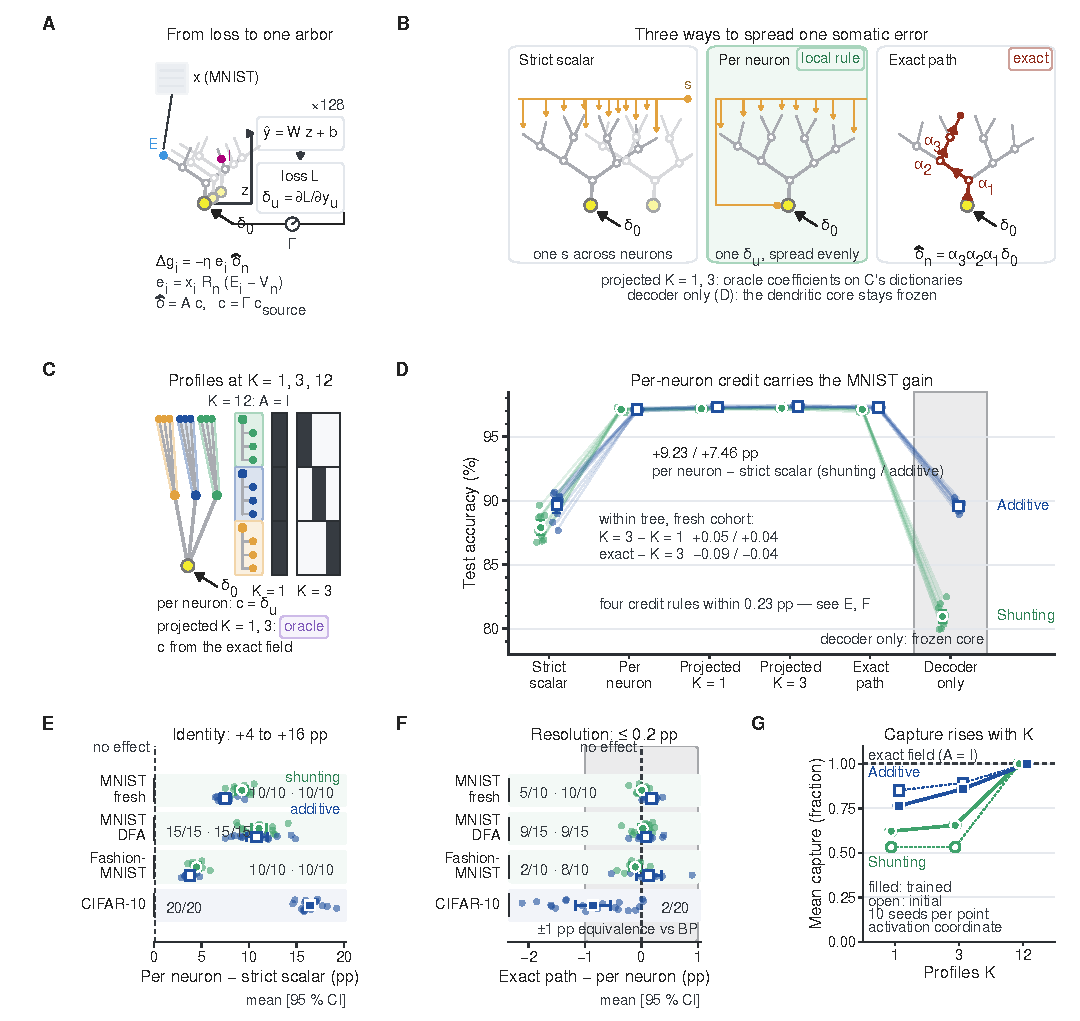
\includegraphics[width=\textwidth]{main/figure_01.pdf}
\caption{\textbf{Task-derived credit separates neuronal identity, spatial address and gain.}
\textbf{A}, A neuron-specific error supplies coefficients $\bm c$; dictionary $A$ and diagonal gains $\Gamma$ give the delivered field $\bm\varepsilon=A\Gamma\bm c$. Synaptic updates multiply credit by local eligibility and negative learning rate.
\textbf{B}, Twelve nonsomatic sites with $K=1$ common, $K=3$ subtree or $K=12$ site profiles. Projected $K=1,3$ rules use oracle activation-error coefficients and retain exact somatic errors.
\textbf{C}, Illustrative projection of a unit-energy gradient with isotropic noise variance $\sigma^2$. A rank-$K$ span retains gradient energy $q$. Twice the smoothness constant $L$ times the optimized one-step progress bound is $q^2/(q+K\sigma^2)$, comparing $(K,q)=(1,0.8)$ and $(2,1)$. This local bound does not predict final trained structure.
\textbf{D}, MNIST with one 128-neuron dendritic layer and a linear readout. Per-neuron credit broadcasts exact somatic activation errors; decoder-only freezes the dendritic core. Lines pair ten fresh seeds per architecture. Rates were selected on three development seeds; checkpoints were validation-selected within 180 epochs.
\textbf{E}, Paired effects of additional spatial resolution in the same cohort.
\textbf{F}, Separate MNIST direct-feedback-alignment (DFA; fifteen seeds) and flattened CIFAR-10 (twenty seeds) controls. Symbols and intervals in \textbf{D--F} show means and descriptive 95\% intervals; colors and shapes identify architectures. pp, percentage points.}
\label{fig:framework}
\end{figure}

\subsection*{Branch-selective information prevents updates from inactive distractors}

To isolate branch-selective information, we used one logistic output with $B\in\{2,4,8\}$ parallel branch weight vectors and no internal forward compartments or conductance nonlinearity (Fig.~\ref{fig:branchconflict}A). Context selected the branch determining the output, while every branch received an image and formed an ungated local eligibility.

Inputs were average-pooled, standardized Fashion-MNIST images from classes 0 and 6. The selected image determined the binary target. At conflict dose \(\chi=0\), all branches received that image; increasing \(\chi\) independently replaced nonselected inputs with opposite-class images. For example \(i\), let \(b_i^\star\) be the selected branch, \(\bm x_{i,b}\) its input vector and \(y_i\in\{0,1\}\) the target. The branch weights \(\bm w_b\) give the pre-probability score (logit) and output error
\begin{equation}
z_i=\bm w_{b_i^\star}^{\mathsf T}\bm x_{i,b_i^\star},
\qquad \delta_i=\sigma(z_i)-y_i.
\label{eq:branchconflictforward}
\end{equation}
Here \(\sigma(z)=1/(1+e^{-z})\) is the logistic function. The exact derivative of every unselected branch is zero, irrespective of its input. Increasing conflict therefore does not create opposing nonzero exact branch gradients. It makes a rule that ignores the selector increasingly sensitive to irrelevant, opposite-class eligibilities.

For \(N\) examples, correctly selected and neuron-shared gradient estimates were
\begin{equation}
\bm d_b^{\rm selected}=N^{-1}\sum_i\delta_i\mathbf{1}[b_i^\star=b]\bm x_{i,b},
\qquad
\bm d_b^{\rm shared}=N^{-1}\sum_i\delta_i B^{-1}\bm x_{i,b}.
\label{eq:branchconflictupdates}
\end{equation}
The indicator $\mathbf{1}[\cdot]$ is one when its condition holds, zero otherwise; $1/B$ matches scale without supplying branch information. A feedback selector and a branch-local eligibility gate give the same update (Fig.~\ref{fig:branchconflict}B), testing access to selection rather than a need for independently computed external errors.

A simplified calculation asks when the selected branch's evidence is outweighed by conflicting evidence sent to other branches. With centered, symmetric class evidence, the shared-mode prediction crosses zero at \(\chi_c=B/[2(B-1)]\): 1, \(2/3\) and \(4/7\) for two, four and eight branches (Fig.~\ref{fig:branchconflict}C; Methods). More branches therefore predict an earlier loss of compatibility. This average calculation is distinct from the conflict dose at which a trained model reaches chance accuracy.

At zero conflict, selected and shared rules achieved similar accuracy. Their difference increased with conflict, reaching 35--58 percentage points at full conflict across the tested branch counts (20 paired seeds; Fig.~\ref{fig:branchconflict}D). In every seed, the advantage of correct routing increased with conflict. A cyclic reassignment sent every signal to the wrong branch at matched rank and sparsity. It was harmful even at zero conflict, reducing accuracy by 12--25 points relative to correct selection. Analytic backpropagation and an explicitly gated grouped-point model matched correct selection exactly, as required by their algebraic equivalence (Fig.~\ref{fig:branchconflict}E; Supplementary Section~S3).

The shared rule reached chance at lower conflict as branch count increased, consistent with the predicted shift (Fig.~\ref{fig:branchconflict}F); five two-branch seeds never crossed in the sampled range. Theoretical, mean-curve and individual-seed crossings are distinct. Gradient alignment also changed during learning (Methods; Supplementary Fig.~S9C--E). Credit reaching inactive branches can therefore harm learning; dendrites offer one possible selection site. A separate two-stream task tests learning and interference effects (Supplementary Fig.~S9A,B).

\begin{figure}[tbp]
\centering
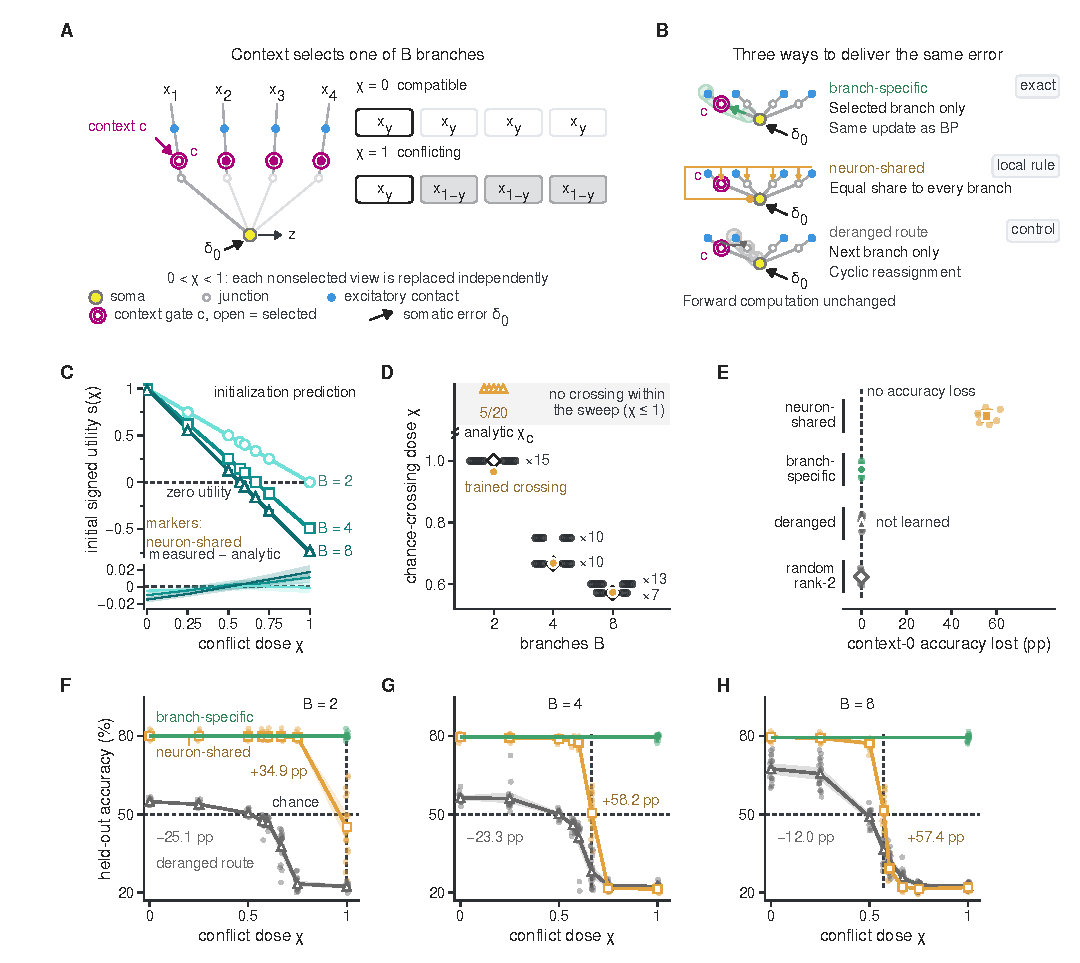
\includegraphics[width=\textwidth]{main/figure_02.pdf}
\caption{\textbf{Branch selection prevents learning from inactive distractors.} One logistic output combines \(B\) parallel branch weight vectors; there are no serial or conductance nonlinearities. \textbf{A}, Context-gated Fashion-MNIST task. Context \(c\) selects the branch determining logit \(z\); every branch receives an image and forms an ungated eligibility. Conflict dose \(\chi\) independently replaces each nonselected image by an opposite-class image. Solid and dashed proximal paths are selected and gated-off forward routes; the double ring marks context. \textbf{B}, Selected feedback: \(\delta_i\mathbf{1}[b=b_i^\star]\), shared feedback: \(\delta_i/B\). Here \(\delta_i\) is the output error, \(b_i^\star\) the selected branch and \(\mathbf{1}\) the indicator; unselected exact derivatives are zero. A local eligibility gate gives the same update. \textbf{C}, Centered symmetric-evidence prediction \(s(\chi)=1-2\chi(B-1)/B\): shared-mode compatibility vanishes at \(\chi_c=B/[2(B-1)]\). This mean-field boundary is distinct from a trained chance crossing. \textbf{D}, Held-out accuracy over conflict dose. \textbf{E}, At full conflict, correct selection, backpropagation (BP) and the algebraically equivalent gated-point calculation coincide; cyclic derangement sends signals to the wrong branch at matched rank and sparsity. Selection-by-conflict interactions are positive in all 20 seeds for each \(B\). \textbf{F}, Analytic threshold (diamonds), first interpolated crossing of mean accuracy (orange), and each seed's first sampled at-or-below-chance dose (faint dots). Open overflow triangles retain five \(B=2\) seeds that do not cross within the sweep. Curves and bars summarize 20 paired seeds with 95\% seed-bootstrap intervals. Branch-count comparisons do not hold capacity fixed.}
\label{fig:branchconflict}
\end{figure}

\subsection*{Ancestry provides a modest advantage at an intermediate feedback budget}

Branch selection compares fully shared with fully resolved feedback. We next asked whether nested subtree routes offer a useful intermediate dictionary. The task contained eight independent, eight-dimensional terminal weight blocks at the leaves of a balanced binary feedback tree. Only the context-selected block determined the logit. Internal tree nodes defined feedback supports and did not perform serial forward computation (Fig.~\ref{fig:subtreefactorial}A).

The selected stream carried the class signal. Distractors carried opposing signals that strengthened with distance through the feedback hierarchy, deliberately favoring task-aligned grouping. At each budget \(K\in\{1,2,4,8\}\), the routing field had \(K\) independent patterns and unit-length rows. Ancestry routes grouped the terminals into the whole tree, halves, sibling pairs or individual terminals. Permuting task streams across leaves changed alignment without changing the streams or forward parameter budget. Here bandwidth counts independent feedback patterns, not physical stages or independent scalar losses; other single-pattern controls need not be uniform. The complete generator and update are given in Methods.

The generator predicts where an intermediate ancestry benefit can occur. The selected stream has class coefficient one; its sibling, same-half nonsiblings and other-half streams have coefficients $-0.15$, $-0.45$ and $-0.75$. The unnormalized sum of the class signal within the selected ancestry group gives $-3.05$, $-0.05$, $0.85$ and $1$ at $K=1,2,4,8$, respectively. Thus coarse pooling reverses or nearly cancels the signal, sibling-pair routing first preserves a positive intermediate-group signal, and full resolution removes the grouping distinction. The implemented unit-row normalization divides these sums by the square root of group size, preserving their signs. This is an analytic consequence of the fixed task design; its location is not an independently discovered optimum (Fig.~\ref{fig:subtreefactorial}B).

Controls preserved rank while changing recipient assignment, support geometry or sparsity: cyclic derangement, depth-interleaving, random-sparse and dense random fields. The per-seed best-control summary takes their maximum after training; it is not a learned selector. A training-informed principal-component reference is retained separately (Methods).

Increasing bandwidth improved correct routing, while derangement caused large losses (Fig.~\ref{fig:subtreefactorial}C). Degree- and depth-preserving rewiring removed the task-aligned advantage at intermediate budgets but did not affect fully shared or fully resolved ancestry routes (Fig.~\ref{fig:subtreefactorial}D). 

The ancestry-specific effect was much smaller. Ancestry performed worse than the best matched control at low budgets, exceeded it by 1.27 percentage points at \(K=4\), and tied at full resolution. The paired \(K=4\) interval was 0.59--1.95 points, with 15/20 positive differences; a paired Wilcoxon signed-rank test gave Holm-adjusted \(P=0.0101\) across four budgets. Individual control contrasts and paired seed differences distinguish this effect from the much larger correct-versus-deranged contrast (Fig.~\ref{fig:subtreefactorial}E,F).

Flat, grouped-point and gated-point representations receiving the same field behaved identically by construction. The experiment therefore supports a conditional advantage of ancestry-shaped feedback under limited bandwidth, without attributing the effect to dendritic material or treating equivalent representations as independent confirmations.

\begin{figure}[tbp]
\centering
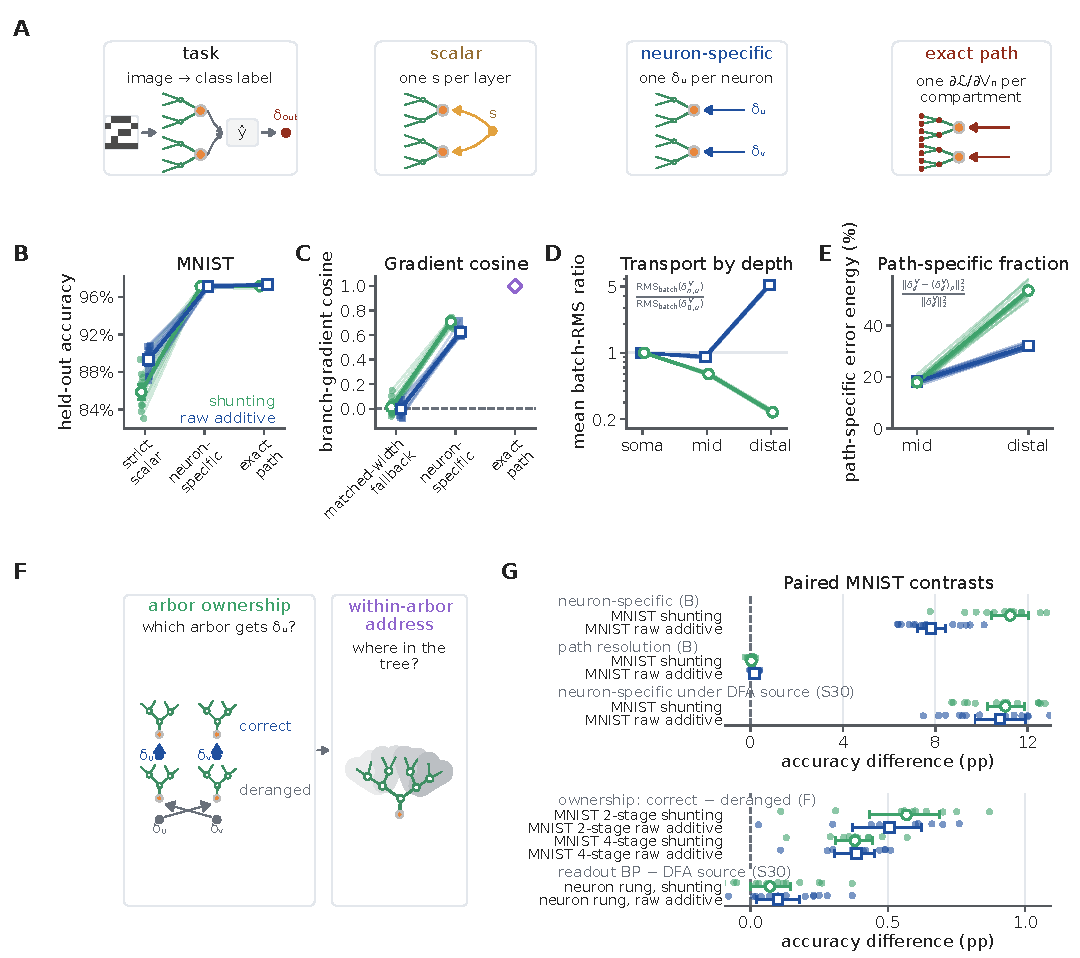
\includegraphics[width=\textwidth]{main/figure_03.pdf}
\caption{\textbf{Hierarchical distractors favor ancestry at intermediate bandwidth.} \textbf{A}, Eight streams carry label sign $s_i$ along noisy teacher features. The selected stream has coefficient one; sibling, same-half and opposite-half distractors have coefficients $-0.15,-0.45,-0.75$. \textbf{B}, Coefficient sums in the cued ancestry group at $K=1,2,4,8$. Implemented feedback divides these sums by square root of group size, preserving their signs. The four-route sign change follows from the design; it is not an independently discovered accuracy optimum. \textbf{C}, Held-out accuracy for correct ancestry, derangement and the per-seed maximum over four matched controls. This maximum is calculated after training, not learned by a selector. Dashed line: chance. \textbf{D}, Task-matched-minus-rewired accuracy at equal degree and depth. \textbf{E}, The four-route ancestry-minus-best-control effect, 1.27 pp (95\% interval, 0.59--1.95), with 15/20 positive seeds and Holm-adjusted two-sided Wilcoxon $P=0.0101$ across four budgets. \textbf{F}, Individual dense, sparse and depth-interleaved contrasts on a separate scale. The large derangement effect is shown in \textbf{C}. Symbols and bars are means and 95\% seed-bootstrap intervals; small points in \textbf{E,F} are twenty paired seeds. Endpoint ties follow from coincident operators.}
\label{fig:subtreefactorial}
\end{figure}

Learning the route coefficients was another limitation. In twenty fresh seeds, an estimator trained on separate noisy context cues improved accuracy over a frozen profile by 7.16 points, but remained 54.47 points below oracle context coefficients. Exploratory selection of its most probable route narrowed the gap, whereas delaying cues removed the benefit (Supplementary Fig.~S10B--D and Section~S3; Methods). These tests expose requirements for selective, timely delivery; they do not derive the context signal from local eligibility.

\subsection*{Cross-branch interactions change the spatial credit that learning uses}

Interactions across branches can change credit's sign and magnitude between examples. We compared targets with identical input-sensitivity spectra on the same representationally compatible tree, separating credit delivery from forward capacity.

Eight independent inputs $x_i$ were equally likely to be $-1$ or $+1$. Each branch computed $u=a+bu_L+cu_R+du_Lu_R$ with four trainable coefficients. This multi-affine unit is affine in either child while the other is fixed. Pairwise targets summed four disjoint products, $f_M=\frac12\sum_{(i,j)\in M}s_{ij}x_ix_j$; quartic targets combined complementary quartets, $f_A=\frac12(s_A\prod_{i\in A}x_i+s_{\bar A}\prod_{i\notin A}x_i)$. Here $M$ partitions inputs into pairs, $A$ is one quartet, $\bar A$ its complement, and signs $s$ were independently sampled. Within each seed, targets shared a compatible balanced tree, input assignment, initial weights and examples (Fig.~\ref{fig:prospective}A). Both have input-sensitivity second moment $\E[\nabla_xf\nabla_xf^{\mathsf T}]=I_8/4$, giving identical strengths of independent sensitivity directions.

Compatibility depends on what each branch must communicate to its parent. Only one scalar leaves a branch, so it cannot transmit several independently required combinations of its inputs. This gives an exact criterion: at each subtree boundary, the matrix of interaction coefficients between inside and outside input products must have rank at most one after removing the constant inside row. The condition is necessary and sufficient across all boundaries; discarded singular values bound representation error (Methods; Supplementary Section~S4).

Logical rules make this forward constraint concrete. All fifteen binary trees over four inputs can represent AND, OR and parity exactly, but mixed rules can require particular input groupings. The rule $(a\,\mathrm{AND}\,b)\,\mathrm{OR}\,(c\,\mathrm{AND}\,d)$ needs only two serial stages, whereas $a\,\mathrm{AND}\,[b\,\mathrm{OR}\,(c\,\mathrm{AND}\,d)]$ needs three in this scalar model, despite containing the same two AND gates and one OR gate. These are exact representability statements, established independently of training (Supplementary Figs.~S13--S14). They connect task composition to possible morphology; the next comparison asks which credit information helps a compatible tree learn.

All credit rules used the same exact local eligibilities and scalar output error. We compared exact paths with unit broadcast and a fixed six-site profile calibrated from each student's mean path derivatives over 256 unlabeled initialization examples. Three development seeds selected learning rates with equal budgets; twenty fresh paired seeds tested the frozen choices. A separate nested target summed products over prefixes of two, four, six and eight inputs on its own compatible tree.

The initially calibrated profile supported pairwise learning but remained inaccurate on quartic and nested targets (Fig.~\ref{fig:prospective}B--D). At the primary 1,024-step checkpoint, mean normalized mean squared errors (NMSE) for exact and calibrated credit were 0.0317 and 0.0236 on pairwise targets, 0.1516 and 0.9813 on quartic targets, and 0.0230 and 0.7690 on nested targets. NMSE divides squared prediction error by clean target variance. The predefined quartic-minus-pairwise difference in calibrated-minus-exact gaps was 0.838 (95\% paired interval, 0.719--0.931), positive in all twenty seeds; a common learning rate gave 0.843 (0.727--0.935). Exact quartic learning was heterogeneous at this checkpoint: seventeen fits were near the noise floor and three remained stalled. The lower pairwise mean for calibrated credit likewise reflected one slow exact fit; exact credit performed better in fifteen of twenty seeds (Supplementary Figs.~S15--S16).

Continuing every algebraic trajectory to 16,384 updates without retuning clarified the sustained comparison. All twenty selected-rate Adam exact quartic fits reached the noise floor by 4,096 updates, and the pairwise mean lag disappeared. At 16,384 updates, the quartic-minus-pairwise calibrated-credit deficit was 0.952 (95\% paired interval, 0.883--1.012) at terminal states and 0.790 (0.691--0.880) under validation-based selection, positive in all twenty seeds (Fig.~\ref{fig:prospective}E). These continuations describe the same previously observed seeds under the same bounded dynamics: fixed-profile arms contacted coefficient bounds, whereas exact arms did not. Common-rate, per-seed, optimizer and bound controls are reported together in the Supplementary Information (Supplementary Figs.~S15--S16 and Table~S8).

The trained fields reveal a distinction missed by the input spectrum. Let $\bm q(x)$ contain the six nonsomatic derivatives of root output with respect to branch output; exact branch credit is scalar output error times $\bm q$. At the 1,024-step checkpoint, allowing an oracle amplitude per example, the best fixed profile captured 99.7\% of exact-trained path-field energy for pairwise targets, but 46.1\% for quartic and 44.8\% for nested targets. The separation persisted at 16,384 updates: capture was approximately 100\%, 39.6\% and 40.5\%, respectively (Fig.~\ref{fig:prospective}F). Loss-error weighting, eligibility weighting, site-normalized spectra and replay of 600 earlier fits preserved the original separation (Supplementary Section~S4). Uniform-profile capture did not: a nearly one-dimensional field can have a signed, nonuniform direction. Positive fixed-profile scaling largely cancels in Adam, explaining calibrated/sign-only agreement; it does not explain the slower pairwise learning with changing exact paths.

Thus input-matched targets developed different credit spectra and tolerance of fixed profiles. At fixed weights and inputs, however, path derivatives are target-independent: their spectrum describes learned states and coordinates, not a task-only initialization diagnostic. Failure of the tested profiles supports example-dependent spatial credit without establishing that six independent channels or exact gradients are necessary.

Additional controls delimit the result. Fixed-profile Adam learned a compatible positive-conductance teacher accurately; broadcast learned aligned XOR-of-AND, whereas parity favored exact credit under the tested optimizer (Supplementary Figs.~S13--S14 and S17). Noisy-query interaction estimation also yielded useful trees, retained as supporting structure-design evidence in Supplementary Fig.~S35. Interaction structure therefore motivates specific credit comparisons rather than a universal monotonic resolution law.

\begin{figure}[tbp]
\centering
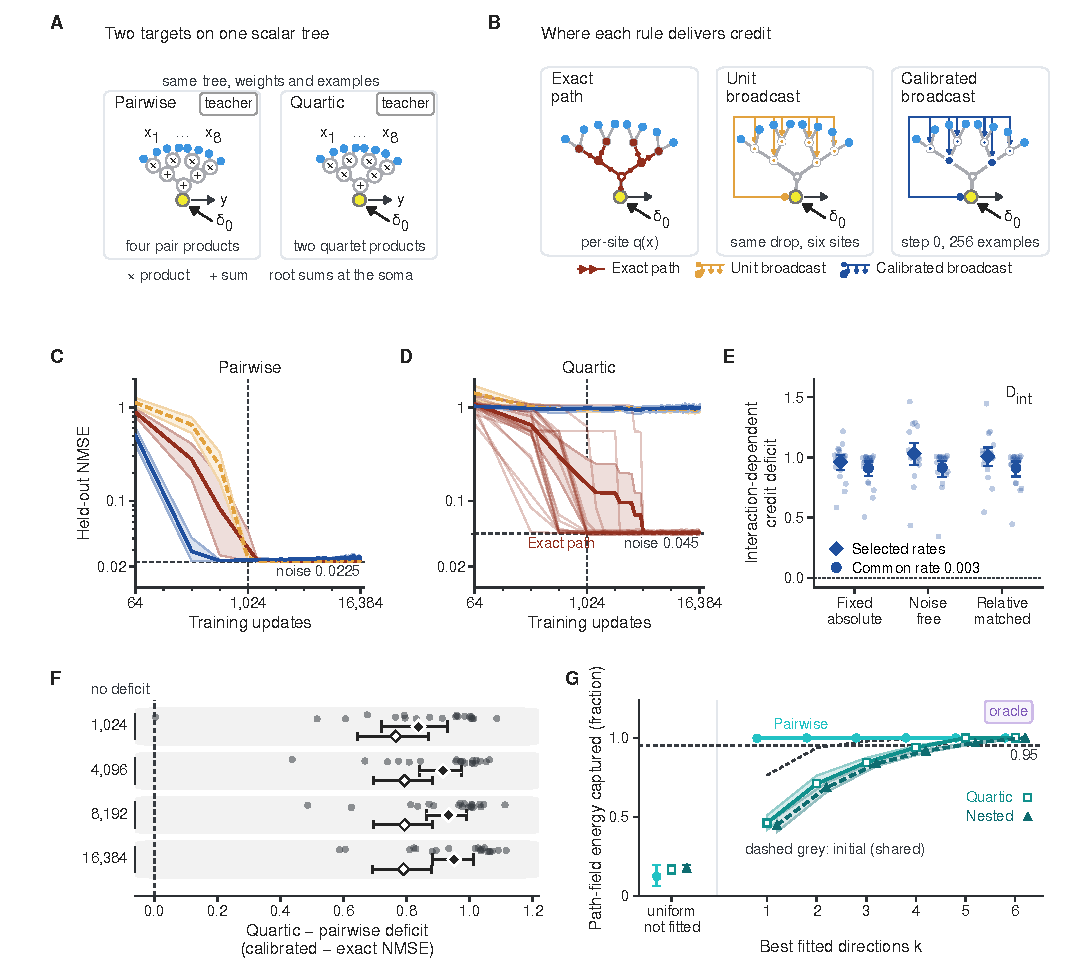
\includegraphics[width=\textwidth]{main/figure_04.pdf}
\caption{\textbf{Matched input spectra yield different learned credit geometry and tolerance of fixed profiles.}
\textbf{A}, Pairwise and quartic targets share eight inputs, a compatible tree, initialization and examples. Signed coefficients have magnitude 0.5; both targets have input-sensitivity second moment $I_8/4$. Nodes illustrate interaction supports.
\textbf{B--D}, Held-out normalized mean squared error (NMSE) for exact credit, unit broadcast and an initial profile calibrated on 256 unlabeled examples. Twenty seed blocks continue to 16,384 updates at the original development-selected Adam rates and coefficient bounds. Nested targets use a separate compatible tree. Curves are current-state means; shading shows pointwise descriptive 95\% whole-seed intervals. Vertical lines mark the primary 1,024-step checkpoint; horizontal lines mark noise-only NMSE (0.0225 for pairwise/nested, 0.045 for quartic).
\textbf{E}, Quartic-minus-pairwise difference in calibrated-minus-exact NMSE at current states and minimum-validation-error states within each budget, with paired 95\% intervals. These continuations use previously observed seeds without retuning.
\textbf{F}, Best rank-one capture of six-site exact path-field energy at initialization, 1,024 and 16,384 updates, with twenty-seed 95\% intervals. The primary and continued checkpoints remain distinct; spatial directions and example-specific amplitudes are oracle fits.}
\label{fig:prospective}
\end{figure}

\subsection*{Context-dependent branch tuning makes spatial credit useful in conductance trees}

We next tested how branch tuning affects credit demand in a conductance tree. A first seven-compartment construction with monotonic branch responses was learned accurately by all tested rules. Under Adam, mean broadcast NMSE remained below 0.0006 after extended training despite a varying path field (Supplementary Fig.~S18). We therefore tested a separate construction in which context selected branches with either aligned or opposing feature tuning (Fig.~\ref{fig:conductancecredit}A,B).

Four terminal compartments fed two proximal compartments and a soma, using the directed E/I conductance balance (Methods). Both subtrees received the same positive feature pairs, $\exp(z_j)$ and $\exp(-z_j)$, for two independent latent inputs $z_j$. A binary context increased inhibitory conductance in one proximal compartment. Teacher excitation and inhibition produced increasing feature responses in both subtrees for the aligned task, but increasing responses in one and decreasing responses in the other for the opposed task. Teacher and student shared the circuit, ensuring representability. Students shared the teacher's nominal proximal and coupling gains, with independent Gaussian perturbations of SD 0.4 in log conductance; terminal gains started near one. All 24 conductances were plastic, and paired conditions shared initial weights and example streams.

At fixed weights, binary context generates at most two exact path profiles. Their gains are positive: context changes the relative weighting of the two distal subtrees, while proximal credit is context invariant. The nominal parent's conductance denominator changes by approximately eightfold. Thus branch selection is the relevant distinction, connecting this task to Fig.~\ref{fig:branchconflict}.

We tested whether that distinction requires oracle coefficients. A local rule delivered the somatic error to terminal parameters only when their parent was uninhibited, while retaining ungated error at proximal compartments and the soma. It used the supplied inhibitory context and exact local eligibilities, without evaluating exact paths or projecting an exact field. Two fixed distal profiles with oracle amplitudes and unit proximal credit supplied a separate capacity control. An additional proximal profile in the earlier three-profile control therefore addresses proximal updates, rather than another context distinction.

After exploratory panel results motivated this rule, we froze its protocol and tested twenty new paired seeds. All nine rules ran at three common rates through 16,384 updates; the primary rate and 4,096-update window were fixed before these outcomes. On opposed targets, mean held-out NMSE was $2.18\times10^{-5}$ for exact credit, $2.33\times10^{-5}$ for the local gate, $2.28\times10^{-5}$ for the two-profile oracle with unit proximal credit, and 0.487 for broadcast (Fig.~\ref{fig:conductancecredit}C,D). On aligned targets, the corresponding exact, local-gate and broadcast errors were $7.53\times10^{-6}$, $1.06\times10^{-5}$ and $5.53\times10^{-4}$. The opposed-minus-aligned difference in broadcast-minus-gate error was 0.487 (95\% paired interval, 0.360--0.615), positive in all twenty seeds. It remained 0.468 (0.332--0.604) within the longer window (Fig.~\ref{fig:conductancecredit}E).

The controls identify what the gate must preserve. Reversing its distal selection gave opposed-task NMSE 0.949. Applying it at proximal compartments as well gave 0.123 and prevented both proximal inhibitory gains from learning: their eligibility is nonzero only during inhibition, precisely when that gate closes (Fig.~\ref{fig:conductancecredit}F). The proper local rule changed all 24 parameters and succeeded across the three tested rates. A continuous shunt-proportional distal gate also worked (Supplementary Fig.~S20).

This success is consistent with coarsening the exact rule's strong context-dependent gain ratio. Earlier same-state gradient diagnostics showed that broadcast mixes opposing context-conditioned updates, despite nonnegative per-example alignment with exact gradients (Supplementary Section~S5 and Source Data). The result establishes a local implementation when inhibitory context and somatic error are supplied; it does not explain their biological origin. All comparisons remain finite-budget and bounded-parameter results. Exact and local-gate fits did not reach conductance bounds, whereas most opposed broadcast fits did; the earlier wide-bound and rate controls remain in Supplementary Fig.~S19.

\begin{figure}[tbp]
\centering
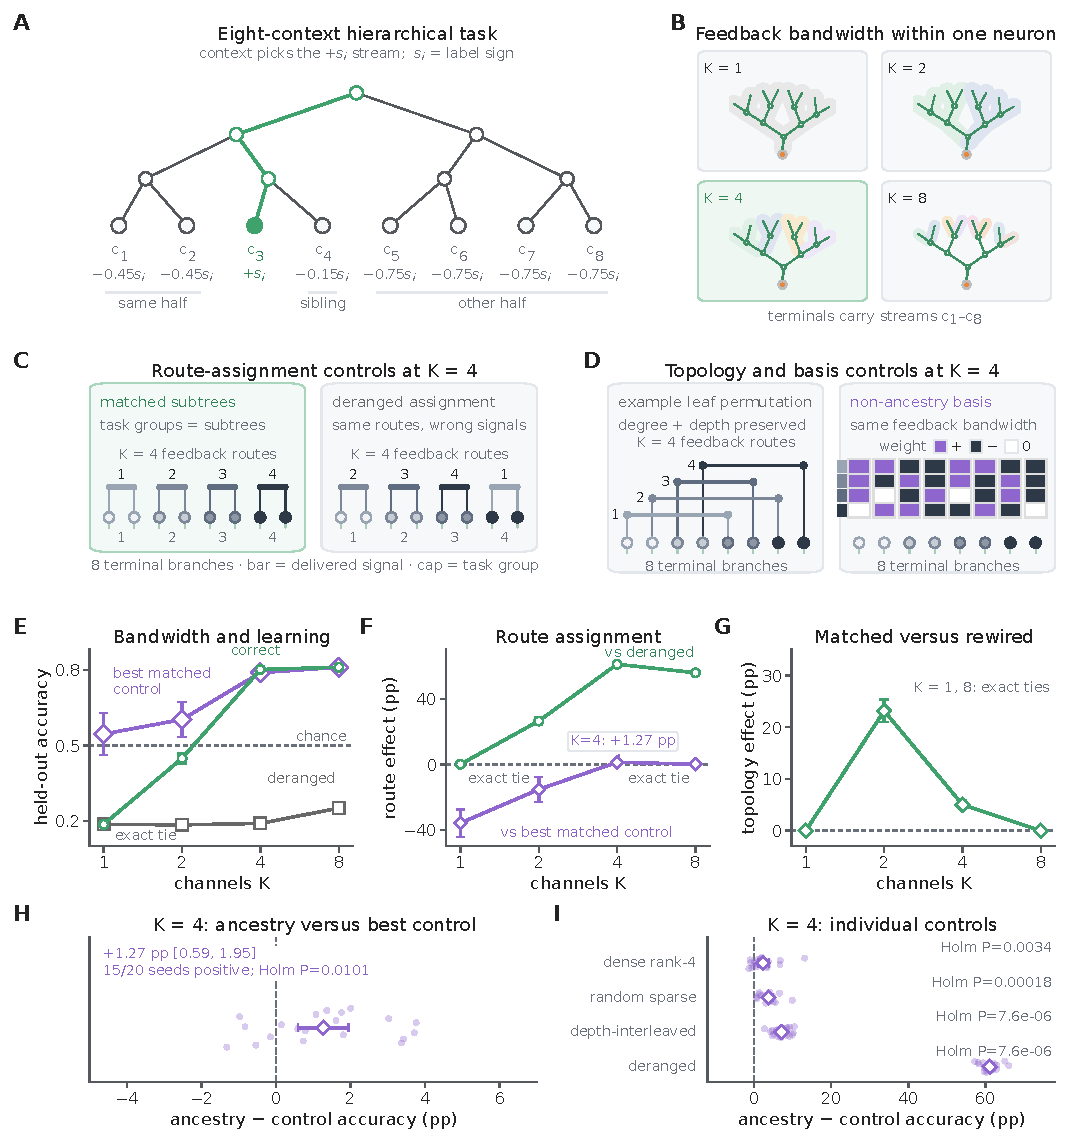
\includegraphics[width=\textwidth]{main/figure_05.pdf}
\caption{\textbf{A local inhibitory gate supplies useful branch selection in a conductance tree.}
\textbf{A}, Four terminal compartments feed two proximal compartments and a soma. All 24 conductances are plastic. The local rule gates terminal credit by the parent's inhibitory activity while retaining unit multipliers for proximal and somatic credit. Local eligibilities are unchanged.
\textbf{B}, Nominal teacher tuning for aligned and opposed branches; both tasks receive identical positive feature pairs.
\textbf{C,D}, Fixed-checkpoint test NMSE for aligned and opposed targets, respectively. Twenty new paired seeds share initial students and example streams across rules. Adam rate 0.03 and both budgets were fixed before execution. The two-profile control uses oracle distal amplitudes and unit proximal credit. Dotted lines mark 4,096 updates; every trajectory continues to 16,384. Update axes are linear through 64 and logarithmic thereafter.
\textbf{E}, Opposed-minus-aligned difference in broadcast-minus-local-gate NMSE, evaluated at minimum-validation-error states within each budget.
\textbf{F}, Opposed-task outcomes within the primary window for correct, swapped and proximal-gated rules. Gating proximal credit freezes two inhibitory gains. Points show every seed; larger symbols and bands in \textbf{C--F} show means and descriptive 95\% whole-seed bootstrap intervals. All rates and nine rules are retained in Supplementary Fig.~S20. Earlier exploratory gate runs are excluded.}
\label{fig:conductancecredit}
\end{figure}

\subsection*{Task organization determines the benefit of serial dendritic computation}

The interaction comparison holds a compatible forward tree fixed while changing credit. We next varied serial forward structure itself, asking whether successive compartments help remove unwanted multiplicative changes in input strength. Physical depth $D_{\rm p}$ counts forward stages, whereas feedback resolution counts distinctions in the backward field.

Each network contained 64 somata and eight nonsomatic compartments per soma. D1 $[8]$, D2 $[2,3]$ and D3 $[2,1,2]$ distributed those compartments across one to three stages in the three- and four-tier comparisons while preserving contacts and trainable resources. The two-tier D2 tree used $[4,1]$, also with eight compartments. Branching vectors are ordered from soma to tips. A resource-identical grouped-point control connected all eight modules directly to the soma; raw-additive trees removed divisive conductance normalization. Flexible point networks provided additional, approximately parameter-matched comparisons.

Distal excitation carried class information multiplied by nuisance gains. Inhibitory sensors reported those gains with alignment $\alpha$: zero retained the sensor distribution but removed trial-specific information, and one reported the factor exactly. With inhibitory reversal zero, the sensors entered the conductance denominator and could support successive divisions \citep{holt1997shunting,carandini2012normalization}. Nested factors acted over fine, coarse and global input groups; flat factors had equal-resolution supports; locally cancellable factors placed the needed ratio within each module (Fig.~\ref{fig:physicaldepth}A). The nested and flat targets involved commutative products. Their distinction was the spatial availability of factor information, rather than a different arithmetic order of multiplication.

In the 180-epoch hierarchy comparison, the two-tier task favored D2, whereas three- and four-tier tasks favored D3 among the tested architectures (Fig.~\ref{fig:physicaldepth}B). The grid was incomplete, and its largest tested means identify budget-specific outcomes rather than a rule equating task tiers with optimal depth. Task-family controls showed what serial organization contributed: at full sensor alignment, exact-BP serial trees exceeded the resource-identical grouped-point control by 30.32 percentage points for nested gains and 22.20 points for flat gains, but had no advantage for locally available ratios. Removing trial-specific sensor information eliminated these large benefits (Fig.~\ref{fig:physicaldepth}C). Serial structure was useful when the task required integrating factor information distributed across modules.

Credit comparisons within this useful forward architecture depended on training duration. Ten paired seeds compared D1 exact BP with five D3 credit/optimization conditions for up to 600 epochs, retaining the original rates, parameter groups and thirty-epoch validation patience. These were matched restarts; the agreement with original-budget fits and complete validation histories are reported in SI. At validation-selected states from the same trajectories, exact-BP D3 exceeded D1 by 30.82 points at 180 epochs and 38.17 at 600 (Fig.~\ref{fig:physicaldepth}D). Eight of ten D1 references stopped early; all fifty D3 fits reached the cap with validation loss still falling. These comparisons establish a forward benefit under the tested budgets, without equating optimization maturity across depths.

Within D3, the LocalCA exact-path-minus-shared-soma accuracy gap changed from $+10.86$ points at 180 epochs to $-1.52$ at 600 (95\% paired interval, $-1.83$ to $-1.23$), with this budget-indexed sign change in all ten seeds. The mean gap remained negative from epoch 315, reached $-2.94$ points at epoch 486, and moved back towards zero by 600 (Fig.~\ref{fig:physicaldepth}E). Exact-path LocalCA nevertheless retained lower mean cross-entropy over epochs 180--600, ending at 0.254 versus 0.276 (Fig.~\ref{fig:physicaldepth}F). Accuracy counts threshold crossings, whereas cross-entropy also reflects predicted probabilities. Under the BP recipe, the 600-epoch exact-minus-broadcast accuracy gap was 0.48 points (0.40--0.55). Thus serial organization and spatial credit answer distinct questions: distributed factor information supports the forward architecture, while the eventual ranking of the tested credit rules remains unresolved (Supplementary Figs.~S21--S23 and Table~S9).

\begin{figure}[tbp]
\centering
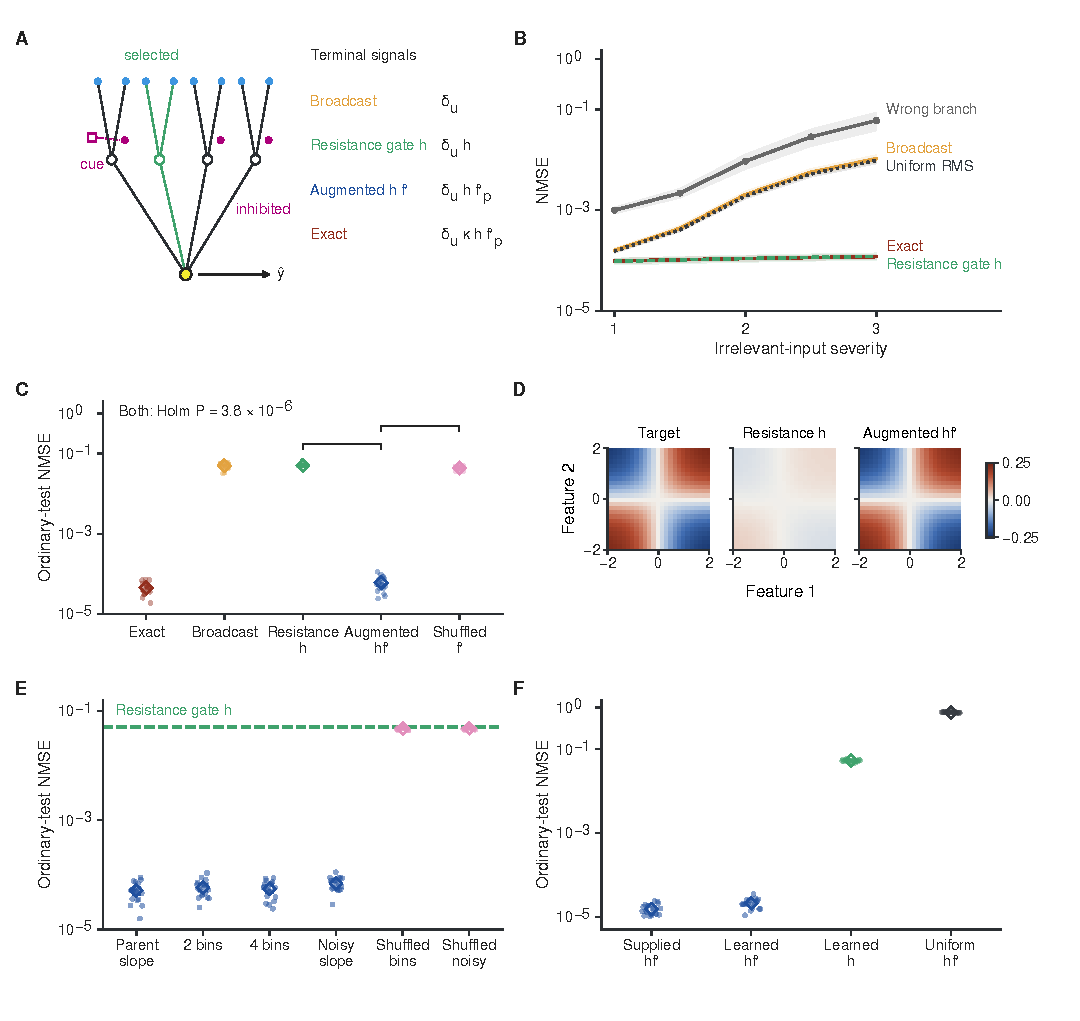
\includegraphics[width=\textwidth]{main/figure_06.pdf}
\caption{\textbf{Task organization determines when serial dendritic computation helps.}
\textbf{A}, Nested gains have fine, coarse and global supports; flat gains have equal-resolution supports; local-ratio tasks expose division within each module. Drawings indicate input access, not exact cancellation. E/I, excitatory/inhibitory inputs.
\textbf{B}, Mean exact-BP accuracy from ten seeds per tested task gain-tier $H$ and physical-depth $D$ combination at 180 epochs. Outlines mark the largest tested means; dashes denote untested combinations. The incomplete grid does not establish converged depth optima.
\textbf{C}, Exact-BP serial-minus-resource-identical-grouped-point accuracy across task families and sensor alignment, with ten paired seeds and 95\% intervals at 180 epochs.
\textbf{D}, Nested-task D1 $[8]$ and D3 $[2,1,2]$ trajectories: 64 somata, eight nonsomatic compartments per soma and matched resources. Validation-selected states are carried forward after stopping.
\textbf{E,F}, Paired D3 exact-minus-shared LocalCA differences in accuracy and cross-entropy. Accuracy changes sign between 180 and 600 epochs; exact credit retains lower mean cross-entropy. All fifty D3 fits reach the 600-epoch cap with falling validation loss; eight of ten D1 references stop earlier. Shading in \textbf{D--F} shows pointwise descriptive 95\% intervals over ten paired seeds. Both recipes use Adam with their original rates and parameter groups; validation selection does not establish convergence.}
\label{fig:physicaldepth}
\end{figure}

\subsection*{Reconstructed arbors provide spatial routes beyond a shared broadcast}

MICrONS links reconstructed anatomy and connectivity to visual responses \citep{microns2025}. We used observed skeletons, soma positions and mapped contact locations and areas to model conductances, voltages and gradient fields, asking whether measured geometry supplies useful delivery patterns. This tests anatomical capacity rather than observed teaching signals.

Each inhibitory-bearing segment supplied a candidate route over its input-bearing descendants (Fig.~\ref{fig:topology}A). Writing these supports as columns connects a branching arbor to a spatial dictionary; an additional constant column supplies a common broadcast (Fig.~\ref{fig:topology}B). For a site-by-route matrix $A_K$, diagonal excitatory-area weights $W$ and weighted least-squares projector $P_{A_K,W}$, capture of a field $\bm t$ was
\begin{equation}
\mathcal C(A_K;\bm t)=\frac{\|P_{A_K,W}\bm t\|_W^2}{\|\bm t\|_W^2},
\qquad \|\bm v\|_W^2=\bm v^{\mathsf T}W\bm v.
\label{eq:reconstructioncapture}
\end{equation}
For an ensemble of perturbations, numerator and denominator sum over field columns. A common-constrained SVD dictionary provided a ceiling at the same column budget. Controls used random anatomical routes, cable-distance bins, site-shuffled routes preserving nonzero counts, and surrogate trees preserving degree and depth while changing ancestry.

The fields were gradient changes induced by small focal shunts in reciprocal cables, generated without inspecting the selected dictionary. They nevertheless favor ancestry by construction: passive transport under a somatic loss has the ancestry structure derived below. This tests how well a small dictionary compresses the tree's own perturbation responses. In the initial eight cells, broadcast captured 31.4\% of field energy, near the 32.6\% rank-one ceiling. Every dictionary therefore contained one common broadcast and $K-1$ spatial profiles, with the protocol fixed before evaluation in 47 disjoint cells from the same mouse and a reconstructed second mouse.

Varying $K$ separates the common signal from the additional spatial information each dictionary can capture (Fig.~\ref{fig:topology}C). At eight columns in the 47-cell cohort, broadcast-plus-ancestry captured 0.619 of total energy versus 0.578 for degree--depth surrogates. The paired advantage was 0.041 (95\% cell-bootstrap interval, 0.020--0.062), positive in 38 of 47 cells. This mean conceals heterogeneity: in 11 cells, more than half of the 200 surrogates matched or exceeded the actual tree. Depth bins captured 0.511 and site-shuffled profiles 0.436; the ancestry-minus-depth difference was 0.108 (0.077--0.135), positive in 45 cells. After removing broadcast, ancestry and depth-bin residual capture was 0.527 and 0.392. The paired residual contrasts show the spatial advantage separately from the shared component (Fig.~\ref{fig:topology}D). Actual ancestry improves average compression within this passive response family, while coarse geometry explains much of the capacity.

Capture and delivery cost are separate constraints (Fig.~\ref{fig:topology}E). The eight-column ancestry dictionary used 18.8\% of the entries of a fully dense dictionary on average; its site-shuffled control preserved exactly the same nonzero count. Equal column count does not ensure equal rank, and nonzero entries are a delivery-cost proxy rather than feedback synapses or metabolic expenditure.

The initial eight cells retained the same ordering (Fig.~\ref{fig:topology}F). In the Pinky second mouse, eight of ten qualifying cells supported the eight-column comparison. Their 9--13 input-bearing sites put ancestry near the residual-capture ceiling, so lower-budget comparisons and exclusions remain separate from the larger arbors. Direct E/I labels covered 4.71\% of disjoint-cohort inputs; the initial cohort's 73.0\% direct-versus-proxy agreement concerned jointly labeled contacts. Geometry, labeling and compression sensitivities accompany the cohort controls in SI (Supplementary Figs.~S24--S27).

\begin{figure}[tbp]
\centering
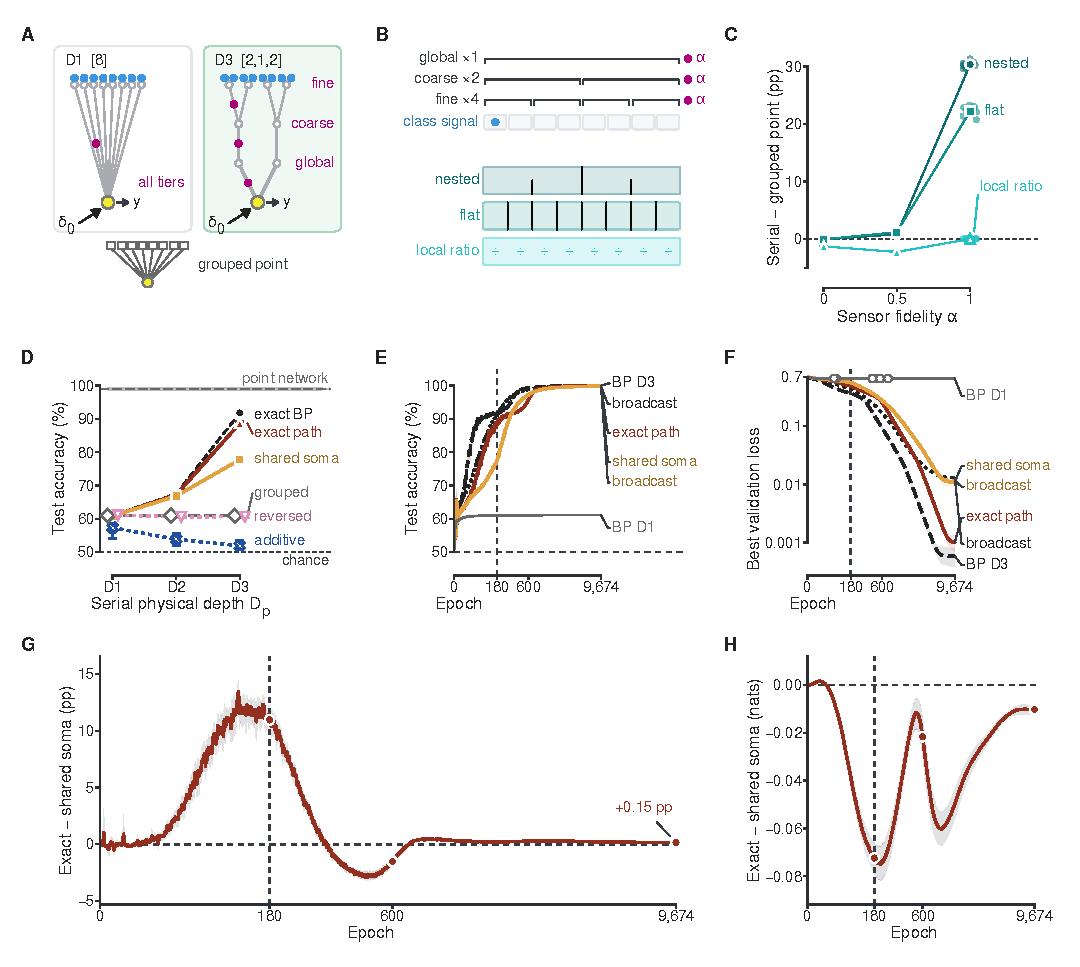
\includegraphics[width=\textwidth]{main/figure_07.pdf}
\caption{\textbf{Anatomy supplies sparse spatial dictionaries beyond a shared broadcast.}
\textbf{A}, Median-sized arbor from the initial eight-cell cohort. Color represents mapped E/I contact-area balance; width represents total contact area. Scale bar, 50~$\mu$m.
\textbf{B}, Illustrative subtree-to-column mapping with a shared constant profile.
\textbf{C}, Capture of field energy remaining after a weighted common projection at $K=1,2,4,8$, each evaluated in all 47 disjoint v661 cells. Every dictionary contains the same constant profile; the common-constrained SVD is an oracle ceiling.
\textbf{D}, Paired ancestry advantages at $K=8$. Surrogate trees preserve segment depths and parent out-degrees; shuffling preserves column nonzero counts. Randomized controls average 200 draws per cell.
\textbf{E}, Residual capture versus mean nonzero coefficient density, relative to dense eight-column wiring. This is a delivery-cost proxy; equal $K$ does not equate rank or wiring.
\textbf{F}, Total and residual ancestry capture in the initial, disjoint and second-mouse cohorts. Pinky's eight eligible cells have only 9--13 input-bearing sites. Symbols and intervals in \textbf{C--F} summarize cell means and descriptive 95\% cell-bootstrap intervals where shown. Capture uses squared excitatory-area-weighted energy. Passive shunt fields inherit ancestry structure through cable physics; this is anatomical compression capacity, not observed teaching.}
\label{fig:topology}
\end{figure}

\subsection*{Focal shunting sets gains on ancestry-defined credit routes}

Morphology supplies spatial routes; conductance can regulate their amplitudes. We examined this connection by comparing a focal inhibitory shunt with a current injection matching its baseline focal current in reconstructed reciprocal cables. A separately solved somatic current restored baseline somatic voltage after either intervention. The endpoint was the change in the modeled excitatory-conductance gradient.

Let \(G\) be the passive conductance matrix and \(\bm b\) the current-source vector, so that baseline voltages satisfy \(G\bm V=\bm b\). With \(\bm e_k\) the unit vector at compartment \(k\), adding inhibitory conductance \(\kappa_k\) at compartment \(k\) changes both \(G\) and its source: \(G'=G+\kappa_k\bm e_k\bm e_k^{\mathsf T}\), \(\bm b'=\bm b+\kappa_kE_{\rm I}\bm e_k\). The matched injection supplies baseline current \(\kappa_k(E_{\rm I}-V_k)\) without changing \(G\). The adjoint $\bm q$ gives loss sensitivity to current injected at each compartment. For a fixed somatic loss derivative, it changes by
\begin{equation}
\bm q'=\bm q-\frac{\kappa_kq_k}{1+\kappa_k(G^{-1})_{kk}}G^{-1}\bm e_k.
\label{eq:sherman}
\end{equation}
The column \(G^{-1}\bm e_k\) gives the voltage response to unit current at \(k\). On a passive tree with a somatic loss, the resulting adjoint change has an exact ancestry structure: all descendants of the shunt share the attenuation factor \([1+\kappa_k(G^{-1})_{kk}]^{-1}\), while each sister block along the path to the soma shares its own factor (Fig.~\ref{fig:focal}A; Supplementary Section~S8). These disjoint blocks form an ancestry partition. Weighting their indicators by the baseline soma-to-site transfer gives a dictionary on which the shunt acts through diagonal gains, providing a physical instance of a diagonal channel-gain matrix, denoted \(\Gamma_u\). The diagonal form applies in this partition basis; it need not hold for an arbitrary selected set of overlapping routes.

In the small-perturbation fields used for Fig.~\ref{fig:topology}, the driving-force term was substantial: its weighted squared energy ranged from 0.99 to 3.50 times that of the full field across the eight initial cells. It opposed the adjoint term (weighted correlations $-0.979$ to $-0.913$). Despite this cancellation, 97.1--99.9\% of full-field energy remained within each focal ancestry partition. The small outside-partition residual therefore does not imply a negligible driving-force contribution (Supplementary Section~S8).

We compared descendants \(D(k)\) with off-route sites \(C(k)\) at similar depth. A separate kernel criterion tests whether the adjoint change is larger below the shunt (Methods); within-cell, reversal-potential and contact-label controls are in Supplementary Fig.~S28B,C.
The analyzed gradient was sensitivity to open excitatory conductance, \(\gamma_i=q_i(E_{\rm E}-V_i)\). The local driving force \(E_{\rm E}-V_i\) can change differently within each block, so the complete synaptic gradient need not share a single block gain. With primes denoting post-intervention values and \(\epsilon_\gamma\) a numerical floor defined in Methods, we measured absolute log change, \(m_i=|\log[(|\gamma_i'|+\epsilon_\gamma)/(|\gamma_i|+\epsilon_\gamma)]|\), and localization \(\Lambda_k=\operatorname{median}_{D(k)}m_i-\operatorname{median}_{C(k)}m_i\). Positive localization means a larger gradient change below the shunt.

In the permissive normalized model, shunts changed descendant gradients more strongly than depth-matched off-route gradients, with increasing localization at higher dose (Fig.~\ref{fig:focal}B; Supplementary Fig.~S28D). Current injection changed descendant gradients roughly threefold less. Its off-route changes were zero by construction under the soma-restoring control; this is not a general claim that current injection cannot change a gradient. Holding the post-shunt voltage but replacing its adjoint with the baseline adjoint removed most localization, supporting a transport contribution beyond the voltage change alone (Fig.~\ref{fig:focal}C).

Physical calibration constrained the spatial selectivity of the gradient change. At axial resistivity \(R_a=150\,\Omega\,\mathrm{cm}\) and specific membrane resistance \(R_m=15{,}000\,\Omega\,\mathrm{cm}^2\), mean shunt-minus-current localization was small and opposite-signed in the initial eight cells and a disjoint 45-cell cohort from the same mouse: \(-0.0019\) and \(+0.0024\), respectively. Signed changes showed attenuation of both descendant and off-route gradients at high resistance; lowering resistance primarily increased descendant attenuation (Fig.~\ref{fig:focal}D). This increased the localization contrast by more than an order of magnitude (Fig.~\ref{fig:focal}E). Distributed background conductance produced the same qualitative recovery at fixed high membrane resistance (Supplementary Section~S8 and Source Data), consistent with a dependence on electrotonic state \citep{chance2002gain,destexhe2003highconductance}.

Adding weak voltage-dependent channel currents produced a dose response close to the passive response at $R_m=1,000\,\Omega\,\mathrm{cm}^2$ with one baseline-leak unit of distributed background conductance (Supplementary Section~S8; Fig.~S29D,E). This checks the local linearization around solved steady states. The baseline Jacobian included gate derivatives but remained fixed across doses, so the check does not establish robustness to strongly active dendrites or channel kinetics.

Together, the exact partition identity and the electrical calibration connect the morphology-defined dictionary to conductance-dependent route gains \citep{gidon2012inhibition}. Their spatial selectivity depends on cable state. These imposed, state-matched perturbations measure modeled transport, rather than endogenous error production, observed plasticity or a learning advantage.

\begin{figure}[tbp]
\centering
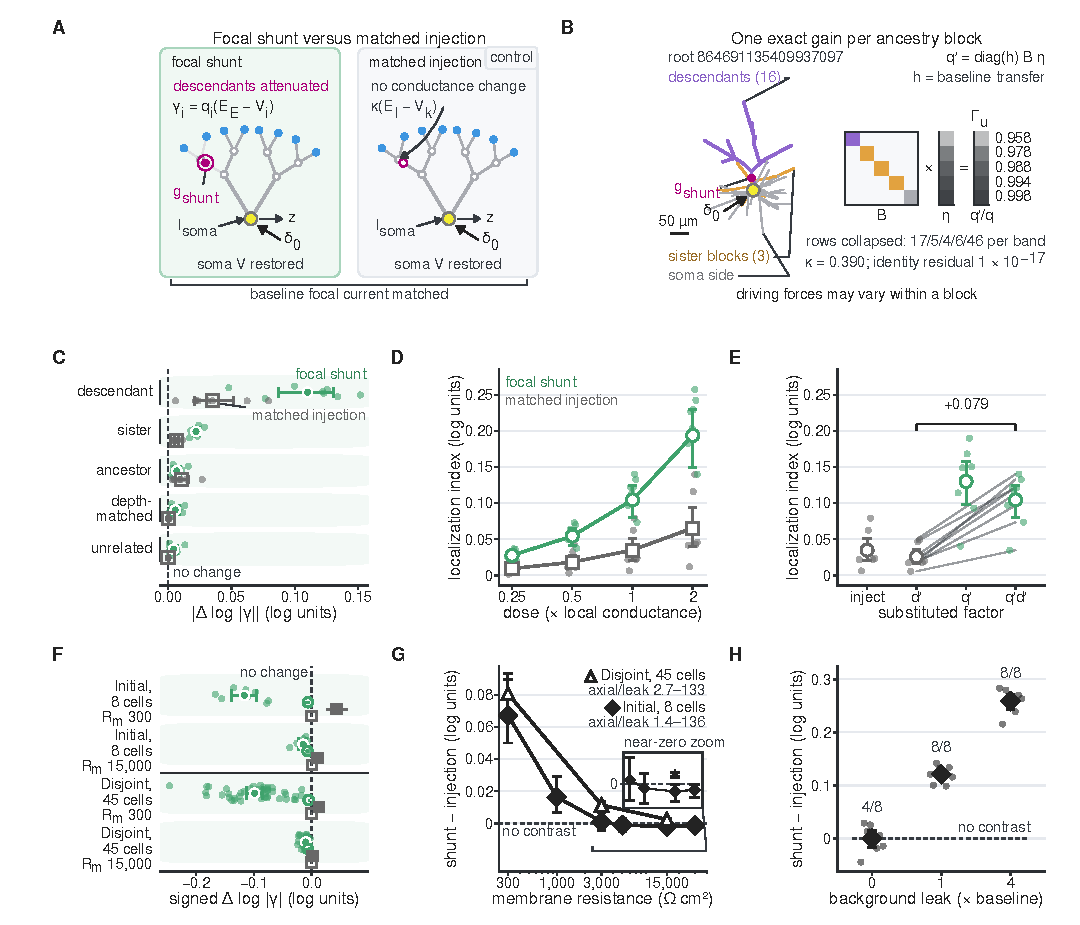
\includegraphics[width=\textwidth]{main/figure_08.pdf}
\caption{\textbf{Focal shunts set ancestry-defined gains whose selectivity depends on electrical state.} \textbf{A}, On a passive tree with a fixed somatic loss derivative, a shunt gives the same adjoint attenuation factor to every site in each colored ancestry block. The resulting gain is diagonal in the baseline-weighted partition dictionary; local synaptic driving forces can still vary within a block. \textbf{B}, Absolute log change in excitatory-conductance gradient magnitude by tree relation at unit dose, in eight reconstructed cells under permissive normalized passive parameters. A current injection matches baseline focal current, and a separately solved somatic current restores baseline somatic voltage after either intervention. Off-route injection zeros arise from this construction. \textbf{C}, Keeping the post-shunt voltage while restoring the baseline adjoint removes most localization. Lines pair cells. \textbf{D}, Signed log change in gradient magnitude at the two physical-calibration endpoints, with \(R_a=150\,\Omega\,\mathrm{cm}\) and \(R_m=300\) or \(15,000\,\Omega\,\mathrm{cm}^2\). Circles and squares show descendants and depth-matched off-route sites; negative values denote attenuation. Site medians are averaged within cells; symbols and whiskers are cohort means and 95\% whole-cell bootstrap intervals (20,000 draws). \textbf{E}, Electrical calibration in the initial eight cells and a disjoint 45-cell cohort from the same mouse. The horizontal axis is the cohort-median axial/leak ratio at fixed axial resistivity \(R_a=150\,\Omega\,\mathrm{cm}\); numerical labels give membrane resistance \(R_m\) in \(\Omega\,\mathrm{cm}^2\). Shunt-minus-current contrasts are small and opposite-signed at \(R_m=15,000\), and increase at lower resistance. Symbols and whiskers are cohort means and 95\% cell-bootstrap intervals after averaging sites within cell. These state-matched perturbations measure modeled transport, not plasticity or learning benefit.}
\label{fig:focal}
\end{figure}

\subsection*{Measured responses bound the anatomical alignment proposal}

The anatomical dictionary and shunt calculations establish capacity and transport. Measured responses ask whether functional relationships preferentially follow ancestry. Seven MICrONS targets had complete arbors and imaged partners: 69 partners in the selected-scan dataset and thirteen eligible scans in the scan-complete analysis. These recordings sampled stimulus responses rather than learning.

Partners with more shared dendritic ancestry did not have reliably more similar condition-mean responses after controlling Euclidean separation and soma-to-contact path-length differences. Mean partial rank correlations were $-0.069$ for selected scans and $-0.048$ for all eligible scans; both target-bootstrap intervals included zero (Fig.~\ref{fig:boundary}A). This test therefore provides no evidence of preferential ancestry alignment in the sampled partners. Its scale differs from population-level like-to-like wiring \citep{ding2025wiring}.

To establish the sensitivity of this small sample, response-level simulations preserved observed partners, shared inputs, repeated stimuli and seven-target inference, with noise calibrated to measured repeat reliabilities. Under the specified Gaussian ancestry-signal model, 80\% detection required a mean simulated target-level partial rank correlation of approximately 0.25 (Fig.~\ref{fig:boundary}B). The observed repeat reliabilities used for attenuation vary across recordings (Fig.~\ref{fig:boundary}C). This conditional threshold leaves weaker effects, different signal geometries and unobserved partners unresolved (Methods; Supplementary Section~S9).

A separate passive-tree model predicted each target's responses from its recorded partners. Its selected ancestry routes reached only 48.0\% of mapped inputs, while one unrestricted fixed transfer profile already reconstructed 98.4\% of exact credit and 97.6\% of exact updates. Restricting that profile to incomplete route supports therefore tests transfer geometry more than example-dependent credit. Mean held-out NMSE was 0.788 for exact learning, 0.803 for ridge regression and 0.832 for the ancestry rule; the ancestry-minus-ridge difference was uncertain (0.029; 95\% target-bootstrap interval, $-0.013$ to 0.074). Allowing oracle coefficients within the same ancestry span barely improved update reconstruction. Full support, prediction, input-removal and reconstruction controls are reported together in the Supplementary Information (Supplementary Figs.~S31--S32). This model diagnostic and the measured ancestry-similarity test constrain different parts of the anatomical proposal.

\begin{figure}[tbp]
\centering
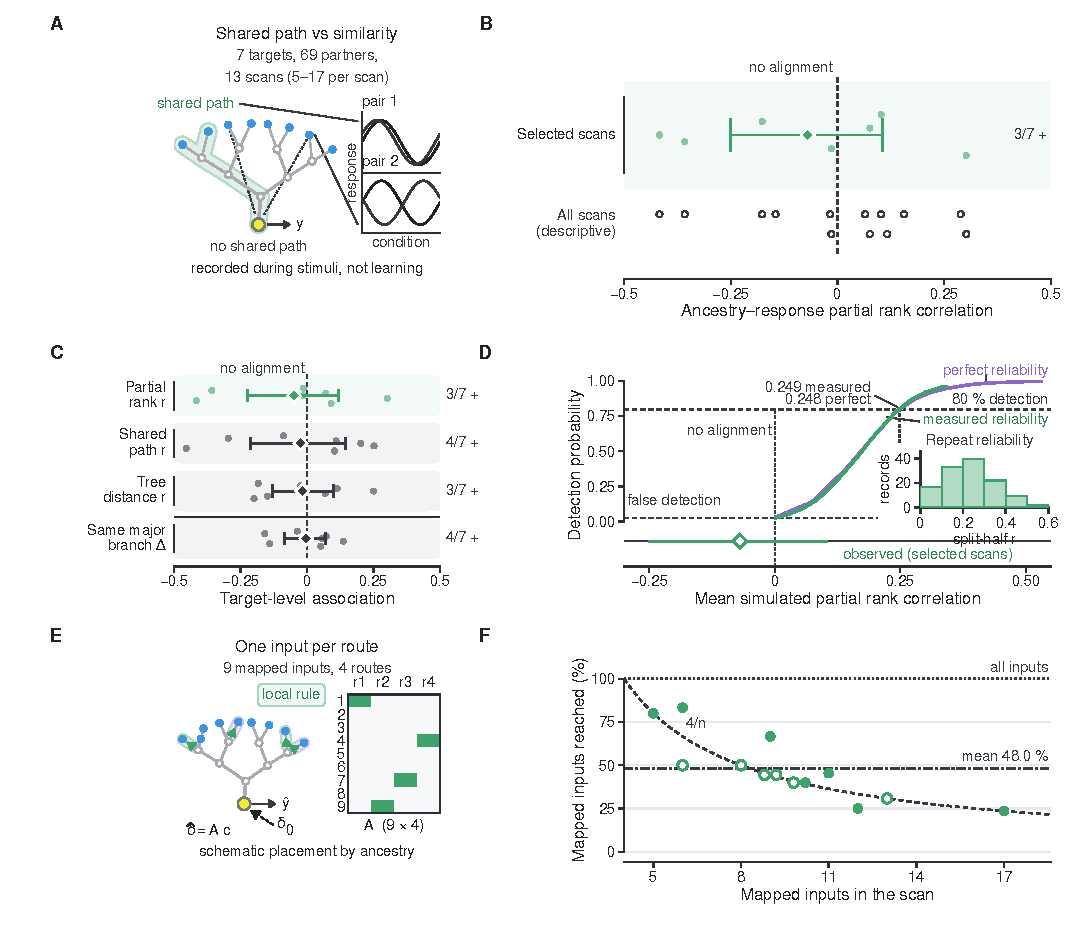
\includegraphics[width=\textwidth]{main/figure_09.pdf}
\caption{\textbf{Measured ancestry alignment and the sensitivity of the available sample.}
\textbf{A}, Ancestry--response partial rank correlations after controlling Euclidean separation and contact-depth differences. Points show seven targets; diamonds and intervals show means and 95\% target-bootstrap intervals. Selected scans contain 69 partners; all eligible scans comprise thirteen scans of the same targets.
\textbf{B}, Conditional positive-alignment detection probability under measured or perfect response reliability. The simulated fraction $\lambda$ allocates latent response variance to a Gaussian ancestry kernel; it is not an observed correlation. Each point summarizes 4,000 datasets analyzed by the exact two-sided seven-target signed-rank test at $P\leq0.05$, also requiring a positive mean. Shading shows 95\% Monte Carlo intervals. With measured reliability, the 80\% threshold lies between $\lambda=0.55$ and $0.60$, corresponding to mean partial correlation approximately 0.25 under this model.
\textbf{C}, Measured split-half response correlations: 125 partner--scan records, 102 unique partners and thirteen scans. Negative values are retained here and clipped to zero only when calibrating nonnegative signal variance in the simulation. Support geometry, ridge comparisons and update reconstruction are reported together in SI.}
\label{fig:boundary}
\end{figure}

\section*{Discussion}

Dendritic trees provide spatial addresses through which learning can distinguish conflicting synaptic demands. Which distinctions are useful depends on the task and the local sensitivity already available to the learner. Morphology supplies delivery patterns, teaching mechanisms supply their coefficients, and conductance regulates their gains. Image learning benefits mainly from preserving neuronal identity, including with random between-neuron feedback. Contextual conflict favors branch selection, supplied through feedback or local eligibility gating. Hierarchical distractors favor ancestry at a bandwidth predicted by the generator's coefficients. These results distinguish useful information from its physical carrier.

The interaction comparison shows why input rank alone is insufficient. Pairwise and quartic targets share input-sensitivity spectra and a compatible tree but develop different credit spectra and tolerance of fixed profiles, despite initial calibration and common-rate controls. Spatial direction matters alongside dimension: even a nearly one-dimensional field can be poorly captured by uniform broadcast. These are learned-state properties, not retrospective support for the failed initialization selector. Intermediate dictionaries, adaptive profiles and alternative dynamics remain plausible solutions.

Conductance trees connect this distinction to a dendritic computation. Simple credit learns some compatible teachers accurately, whereas opposing branch tuning under contextual inhibition benefits from branch selection. A local inhibitory gate supplies that selection without oracle path coefficients, provided proximal credit remains ungated. The task supplies the inhibitory context and somatic error; discovering these signals remains a separate problem. Forward compatibility remains essential: the scalar multi-affine cut criterion connects input grouping to hierarchical tensor descriptions and supports structure estimation from noisy examples \citep{hackbusch2009tensor,grasedyck2010hierarchical,cohen2016tensor}. Serial composition likewise helps remove distributed nuisance factors, but the LocalCA accuracy advantage of exact credit changes sign between the 180- and 600-epoch budgets while exact credit retains lower cross-entropy. The gap is still moving at the cap. Task rank, physical depth and credit resolution therefore describe different constraints.

Obtaining coefficients remains a limitation beyond this explicit context gate. In the separate soft-encoder experiment, the prespecified noisy-cue condition remained 54.47 percentage points below oracle routing (Supplementary Fig.~S10D and Section~S3). Even with sixteen noise-free calibration trials, the encoder identified every context yet achieved only 19.4\% task accuracy; exploratory maximum-probability readout reached the 80.3\% oracle accuracy. This isolates leakage into incompatible routes as a failure mechanism. The exploratory rescue qualifies the primary deficit without replacing it. Exact paths and projected coefficients elsewhere remain information-access controls, and successful routing requires both an adequate span and coefficients that preserve its useful distinctions.

Reconstructed arbors compress their modeled passive response fields beyond a common broadcast. Degree--depth surrogates explain much of this capacity, and the target fields themselves favor ancestry through passive transport under a somatic loss. Testing alignment beyond that construction requires measured fields or a model with different error sources or active dynamics; changing the passive perturbation family alone would not suffice. Focal shunting supplies a biophysical link by reweighting the baseline-weighted ancestry partition. Driving-force changes partly cancel adjoint changes, while cable state sets the spatial selectivity of the resulting gradient. This concerns sensitivity transport, distinct from inhibition that computes errors or regulates forward gain and load \citep{rossbroich2023disinhibitory,galloni2026cellular,greedy2026celltype,safaai2026gainload}.

Measured ancestry--response similarity provided no evidence of preferential alignment in the small recorded cohort. The offline learning comparison chiefly tests preservation of an almost fixed transfer profile and offers limited evidence about endogenous route use. A direct experiment would compare plasticity below a focal inhibitory site with electrotonically matched off-route sites while matching somatic voltage, first-order current and outcome signal. Changing conductance state would test the predicted separation between shared and ancestry-selective effects \citep{francioni2026vectorized,cichon2015branch,bloss2016structured}.

The framework complements somatic prediction, segregated teaching, interneuron-mediated errors and burst plasticity \citep{urbanczik2014dendritic,guerguiev2017segregated,sacramento2018dendritic,payeur2021burst}, alongside cable-learning and engineered gating models \citep{bicknell2021synaptic,chavlis2025dendrites,sezener2021gated,iyer2022activedendrites,lv2025dendritic}. Spikes, temporal eligibility, recurrence and channel kinetics may change the available profiles and coefficient estimation \citep{bittner2017btsp,magee2020plasticity}. The organizing question remains which task-relevant distinctions the arbor and learning mechanism can jointly preserve.

\section*{Methods}

The Methods define the models, task manipulations and inferential units behind the main comparisons. The Supplementary Information's contents and cohort index (Table~S11) locate derivations and complete protocols. Section S1 covers exact and restricted credit; S2--S3 cover images, conflict and ancestry; S4--S6 cover interactions, conductance learning and physical depth; S7--S9 cover anatomy, shunting and measured responses. S10 presents optional structure-selection studies, statistics and reproducibility. Resolved configurations, seeds, checkpoints, exclusions and source hashes accompany the numerical tables. Reusing a cohort for a diagnostic does not add independent observations.

\subsection*{Conductance models and delivery coordinates}

In a directed tree, $[b_1,\ldots,b_D]$ lists branching factors from soma to tips, giving $\sum_{d=1}^D\prod_{r=1}^db_r$ nonsomatic compartments. A child $c$ supplies output $a_c=f_c(V_c)$. With leak $g_n^{\rm L}$, aggregate open excitatory/inhibitory conductances $G_n^X=\sum_{i\in\mathcal S_n^X}g_i^Xx_i^X$ for contact class $X$, and child couplings $g_{c\to n}^{\rm den}$, the steady voltage is
\begin{equation}
V_n=R_n^{\rm tot}\left(g_n^{\rm L}E_{\rm L}+G_n^{\rm E}E_{\rm E}+G_n^{\rm I}E_{\rm I}+\sum_cg_{c\to n}^{\rm den}a_c\right),
\quad (R_n^{\rm tot})^{-1}=g_n^{\rm L}+G_n^{\rm E}+G_n^{\rm I}+\sum_cg_{c\to n}^{\rm den}.
\label{eq:directedvoltage}
\end{equation}
Here $x_i\geq0$ is contact activity, $g_i\geq0$ its conductance, and $E_X$ its reversal potential. A terminal-to-soma pass evaluates the directed steady state. Artificial conductance trees use dimensionless leak one and reversals $E_{\rm L}=E_{\rm I}=0$, $E_{\rm E}=1$. Monotone parameter transforms enforce nonnegative conductances. Branch-output nonlinearities, termed reactivations in the implementation, are identity functions when disabled. Both excitatory and inhibitory contacts learn in the regular-tree experiments.

For a reciprocal cable residual $\bm F(\bm V,\bm g,\bm x)=0$, the nonsingular voltage Jacobian $J_V$ gives the adjoint
\begin{equation}
J_V^{\mathsf T}\bm q=\nabla_{\bm V}\mathcal L,
\qquad \partial\mathcal L/\partial g_i=-\bm q^{\mathsf T}\partial\bm F/\partial g_i.
\label{eq:generaladjoint}
\end{equation}
With passive current balance, the synaptic gradient is $x_i(E_i^{\rm rev}-V_n)q_n$. This established sensitivity calculation supplies the reference for restricted credit \citep{almeida1987asynchronous,pineda1987recurrent,schiess2016somatodendritic,bicknell2021synaptic}. Directed LocalCA combines local eligibility with delivered credit. For output $a_n=f_n(V_n)$, activation error $\delta^a_n=\partial\mathcal L/\partial a_n$ gives voltage error $\delta^V_n=f_n'(V_n)\delta^a_n$. The image implementation retains $f_n'$ in local eligibility and replaces $\delta^a_n$; its gate updates also retain their exact local derivatives. Thus a fixed activation-space profile can correspond to a state-dependent voltage-space profile. Supplying the exact field recovers the exact selected gradients.

The raw-additive control retains the graph but sums signed inputs without the conductance denominator or reversal-potential driving force. Historical normalized-additive controls additionally standardize voltage across stage coordinates within each example; Supplementary Section~S2 defines those variants. The optional four- and five-factor rules add stage-level preconditioners and are described in Supplementary Section~S1.

Writing a delivery dictionary as $A\Gamma$ separates spatial profiles in $A$ from diagonal channel gains in $\Gamma$. Nonzero gains preserve the column span and oracle capture, while changing delivered coefficients and conditioning. A passive focal shunt admits this representation in its baseline-weighted ancestry partition; arbitrary overlapping dictionaries need not. Physical stage count, feedback rank, external error dimension and state-dependent path resolution are distinct resources (Supplementary Tables~S1--S2).

\subsection*{Image feedback ladders and checkpoint diagnostics}

For example $i$, the trained linear decoder supplies activation errors $\delta_{i,u}=\partial\mathcal L/\partial a_{i,0,u}$ at the somatic outputs of neurons $u$. The strict scalar is their mean unless its magnitude is at most $10^{-6}$, in which case it is the largest-magnitude coordinate, preserving that coordinate's sign. The same scalar reaches every core compartment, including the somatic gate. Neuron-specific feedback repeats each neuron's own coordinate throughout its arbor; exact transport multiplies it by the local path derivatives. The historical matched-width fallback retained neuronal identity at the 128-wide somatic stage, affecting 640 of 2,413,312 core parameters. A separately trained strict-scalar control tests that exception (Supplementary Section~S2 and Source Data indexed in Table~S12).

The new MNIST ladder uses 128-soma $[3,3]$ shunting and raw-additive networks, with 40 excitatory and 20 inhibitory contacts per nonsomatic compartment. Within each architecture, rules share initial contact construction, initialization policy, decoder and data streams. Pixels are divided by 255 and flattened without further normalization or augmentation. Each seed divides the 60,000 training images into 48,000 training and 12,000 validation examples; all 10,000 official test images remain held out. Training uses 180 epochs, batches of 256 and the minimum-validation-cross-entropy checkpoint, without early stopping. Adam uses $\beta_1=0.9$, $\beta_2=0.999$, $\epsilon=10^{-8}$ and no weight decay. Original rates are 0.0015 for input synapses and decoder, 0.0007 for branch couplings and 0.0005 for reactivation gates.

Projected $K=1$ averages all twelve nonsomatic activation errors. The $K=3$ dictionary instead averages each proximal compartment with its three distal children. Both use the exact field and preserve its mean at identical weights; their norms can differ. Both projected rules retain exact somatic errors and local activation derivatives. A decoder-only reference trains the readout on the initialized core, whose unchanged hash is verified. Three development seeds compare rate multipliers 0.3, 1 and 3 for every rule and architecture, giving 108 fits. Validation alone selects rates. Ten fresh paired seeds per architecture and rule give 120 selected-rate and 120 original-common-rate outcomes from 190 unique fits; 50 fits serve both policies. The projected-$K=1$ addendum was frozen before fresh outcomes. Complete protocols, clipping and excluded implementation checks are in Supplementary Section~S2.

The original fifteen-seed MNIST ladder is retained in Supplementary Section~S2 and Source Data; its gradient diagnostics appear in Fig.~S7E--G. Fashion-MNIST uses ten paired seeds; the raw-additive CIFAR-10 ladder uses twenty and a 20-soma $[3,3,3,3]$ tree. Their distinct protocols and initialization are retained in SI. The separate fifteen-seed direct-feedback-alignment factorial replaces the decoder derivative by a fixed Gaussian output-to-neuron matrix, scaled by inverse square root of output dimension. It pairs random-feedback fits with the original exact-readout reference. Ownership controls permute neuronal recipients without changing coordinate values or bandwidth.

Common-checkpoint diagnostics compare rules at identical weights and states. Exact path transport is checked against automatic differentiation. New capture measurements use 2,048 held-out images at initial and exact-trained states; activation- and voltage-space metrics are kept separate. Gradient cosine, error magnitude by depth and mean-subtracted path energy are distinct summaries; none alone certifies learning performance. Historical depth and noise cohorts, including their task-identity and conductance-validity records, are specified in Supplementary Section~S2.

\subsection*{Contextual conflict and ancestry routing}

In the branch-conflict task, one context-selected branch determines a logistic output while all $B$ branches form ungated local eligibilities. Nonselected Fashion-MNIST views are replaced independently by opposite-class images with probability $\chi$. Exact feedback is $\delta_i\mathbf1[b=b_i^\star]$; shared feedback is $\delta_i/B$, where $\delta_i$ is output error and $b_i^\star$ the selected branch. Twenty paired seeds cross $B=2,4,8$ with eight conflict doses. The algebraically equivalent gated-point calculation and BP receive the same updates; cyclic derangement preserves rank and support while changing the recipient.

Under centered, symmetric class evidence, shared-mode compatibility is $s(\chi)=1-2\chi(B-1)/B$, with zero at $\chi_c=B/[2(B-1)]$. This mean-field prediction is separate from a trained accuracy crossing. The latter is reported both by interpolation of the mean curve and by each seed's first sampled at-or-below-chance dose, retaining non-crossings. Checkpoint re-execution reproduces endpoints and compares exact/shared fields at both common and own trained states (Supplementary Fig.~S9C--E).

The ancestry factorial contains eight eight-dimensional blocks. Context $c_i$ and binary label sign $s_i$ are balanced, and inputs are $\bm x_{i,b}=a(b,c_i)s_i\bm t_b+\bm\epsilon_{i,b}$, with seed-specific unit teachers $\bm t_b$ and Gaussian noise $\bm\epsilon_{i,b}\sim\mathcal N(0,1.1^2I_8)$. The selected coefficient is one; sibling, same-half nonsibling and opposite-half coefficients are $-0.15,-0.45,-0.75$. A leaf permutation changes task-to-route alignment without changing the streams. For budget $K$, ancestry feedback has context-by-block entries $\Phi^{(K)}_{cb}=\sqrt{K/8}\,\mathbf1[g_K(\pi(c))=g_K(b)]$, where $g_K$ indexes contiguous groups and $\pi$ maps streams to leaves. Thus every row has unit Euclidean norm.

The update is $\Delta\bm w_b=-(8\eta/N)\sum_i\delta_i\Phi^{(K)}_{c_ib}\bm x_{i,\pi^{-1}(b)}$, with $N$ training examples and rate $\eta$. Each seed supplies 2,048 training, 2,048 test and 1,024 switch examples. Full-batch descent uses rate 0.3, eighty training epochs and twenty switch epochs. Controls include deranged ancestry, depth-interleaved and random-sparse supports, dense rank-$K$ fields and a training-informed PCA reference. The best matched control is the per-seed post-training maximum over the four non-PCA controls. Integer test counts preserve ties in the named Wilcoxon comparison; Holm correction covers four budgets. Alternative mean-sign-flip and historical BH analyses remain explicitly labeled in the Source Data indexed in Supplementary Table~S12. The separate noisy-context encoder and cue-delay experiments are fully specified in Supplementary Section~S3.

\subsection*{Update utility and prospective selection}

Let the exact gradient be $\bm\mu$ and the delivered update estimator have mean $\bm m$ and covariance $\Sigma_{\rm route}$ at the current weights. For an $L$-smooth loss and a nonnegative step $\eta$, expected loss after the update is bounded above by $\mathcal L-\eta\bm\mu^{\mathsf T}\bm m+(L\eta^2/2)(\|\bm m\|^2+\operatorname{tr}\Sigma_{\rm route})$. Optimizing this expression gives utility $U=[\bm\mu^{\mathsf T}\bm m]_+^2/[2L(\|\bm m\|^2+\operatorname{tr}\Sigma_{\rm route})]$, with zero for a zero denominator. Utility certifies one-step progress under the stated moments; it is not a long-horizon ordering.

Synthetic quadratic screens isolate signal retention, noise rejection and fixed gains over sixteen Haar coordinates, without a forward neuron (Supplementary Fig.~S2). Their matched signal/noise hierarchy is a designed crossover. The trained factorial's retrospective utility uses actual full-batch updates and a global logistic-curvature bound; choosing maximum bandwidth matches its selection success. The separate prospective linear experiment retains all 12,800 fits, the initialization selector's loss to fixed maximum-budget and rank-only baselines in every seed, and follow-ups forecasting evolving weights and noise. The 25,600-fit dynamics extension and observed-context-count control are reported in Supplementary Figs.~S33--S34, with sealed choices, complete methods and computational costs.

\subsection*{Interaction compatibility, fixed profiles and learned spectra}

For a subtree leaf set $S$, $C_S$ arranges the target's Fourier interaction coefficients by products inside and outside $S$; $C_S^\circ$ removes the constant inside row. Scalar multi-affine trees represent the target exactly if and only if every centered cut has rank at most one. If $\mathcal S(T)$ contains all proper cuts of tree $T$ and singular values are ordered from largest to smallest,
\begin{equation}
\operatorname{MSE}(f,\widehat f_T)\geq B(T;f):=\max_{S\in\mathcal S(T)}\sum_{j\geq2}\sigma_j(C_S^\circ)^2.
\label{eq:morphologyselection}
\end{equation}
Overlapping cut tails cannot be added as a lower bound. Supplementary Section~S4 gives the constructive proof, minimum-depth algorithm and its relation to hierarchical tensor representations. The twelve-tree census, noisy-query estimator, end-to-end learning pipeline, conductance grouping controls and Boolean truth tables remain in Supplementary Figs.~S11, S13--S14, S17 and S35. The theorem's assumptions do not extend automatically to general conductance ancestors.

The matched credit experiment uses twenty fresh seed blocks after three development seeds select rates with equal tuning budgets. Matching and quartic conditions share tree, leaf assignment, initialization, inputs, additive noise and minibatch order. Exact, unit, initially calibrated and sign-only profiles use the same local eligibilities; calibration averages initial path derivatives over 256 unlabeled examples. Selected and common-rate outcomes are retained for SGD and Adam, giving 432 development and 1,200 fresh fits. Algebraic coefficients remain within $[-2,2]$, and all bound contacts are recorded. The original fits stopped at 1,024 steps with seven saved checkpoints. A balanced extension retained all 720 unique algebraic trajectories at the selected/common-rate union, replayed every original checkpoint and continued to 16,384 steps. Its terminal and validation-selected results are descriptive analyses of the same seeds (Supplementary Section~S4). Noisy held-out NMSE divides by clean target variance: one for matching and nested, one-half for quartic. All have noise variance 0.0225. The primary Adam contrast subtracts the pairwise calibrated-minus-exact gap from its quartic counterpart.

For evaluation-example-by-site path matrix $Q$, the best fixed profile is the leading right singular vector. Its capture is $\sigma_1(Q)^2/\sum_j\sigma_j(Q)^2$, an oracle reconstruction with example-dependent amplitudes. Additional diagnostics evaluate uniform, calibrated and ancestry profiles, loss-residual weighting, eligibility-weighted updates and root-mean-square normalization of each site. Participation-ratio effective rank is $(\operatorname{tr}C)^2/\operatorname{tr}(C^2)$ for uncentered $C=Q^{\mathsf T}Q/N$. At fixed weights and inputs, changing labels leaves the path field unchanged; eighty relabeling controls verify this. Independent checkpoint analysis and faithful replay of 600 earlier fits provide numerical and trajectory checks. Complete definitions, pairing audits, optimizer effects and the positive-conductance boundary are in Supplementary Sections~S4--S5.

\subsection*{Conductance trees with context-dependent feature tuning}

The seven-compartment model uses identity branch outputs in Eq.~\ref{eq:directedvoltage}. Two independent $z_j\sim\mathcal U[-2,2]$ generate positive inputs $\exp(\pm z_j)$ for both subtrees. Every terminal has two excitatory and two inhibitory gains; binary context inhibits one proximal compartment. All 24 conductances are positive and parameterized by logarithms. Students start from terminal gains one, proximal inhibitory gains 15, daughter couplings 20 and 0.2 per subtree, and soma couplings four. These proximal and coupling values match the teacher's nominal scaffold, not its realized weights. Independent Gaussian log perturbations have SD 0.4 in students and 0.15 in teachers. Full generators and eligibility derivatives are given in Supplementary Section~S5.

The local-gate follow-up used twenty new paired seeds and nine rules at Adam rates 0.01, 0.03 and 0.1, giving 1,080 trajectories. Each task supplied 2,048 training, 1,024 validation, 4,096 test and 512 unlabeled calibration examples. The primary rate 0.03 was fixed from earlier work, not selected on these seeds. Minibatches contained 128 examples; logarithmic conductances stayed within $[-7,7]$. Minimum validation NMSE selected states within fixed 4,096- and 16,384-update windows. The somatic error was $(V_s-y)/\operatorname{Var}_{\rm train}(y)$; NMSE uses clean target variance. At a terminal with parent $p$, the hard gate multiplied this error by $\bm1[a_p=0]$, where proximal inhibitory activity $a_p$ was zero or ten. Proximal and somatic multipliers remained one. The continuous gate used $1/(1+g_p^{\rm I}a_p)$. Both combined these signals with the same exact local eligibilities and accessed no exact path derivatives.

Controls used exact credit, unit and initially calibrated broadcast, two weighted distal oracle profiles with unit proximal credit, three oracle profiles including a proximal column, reversed distal gating, and gating at proximal sites as well. Two primary paired sign-flip tests---opposed broadcast-minus-gate error and its opposed-minus-aligned difference---were Holm-adjusted together. Other comparisons and 95\% whole-seed bootstrap intervals were descriptive. The protocol was committed after exposure to exploratory panel results but before execution on the new seeds. Earlier development, wider-bound controls and new local-gate controls are in Supplementary Figs.~S18--S20. Full rule definitions, gradient-cancellation diagnostics, validation and outcomes are retained in Supplementary Section~S5 and its Source Data.

\subsection*{Serial depth, sensor alignment and optimization}

Physical-depth networks contain 64 somata and eight nonsomatic modules each. D1--D4 reallocate these modules across branching vectors $[8]$, $[2,3]$, $[2,1,2]$ and $[1,1,2,2]$ in the three- and four-tier comparisons; the two-tier D2 tree uses $[4,1]$. Contacts and resources are matched; serial composition changes. Grouped-point controls connect every module directly to the soma. Raw-additive controls retain the graph without division, while flexible MLP controls are approximately parameter matched.

Excitatory blocks carry class evidence multiplied by lognormal nuisance factors. Inhibitory blocks sense those factors with alignment $\alpha$: zero removes trial-specific information while preserving the sensor distribution, and one reports the factor. The generator floors noisy input rates before multiplying them by gains. Nested, flat and local-ratio families distinguish distributed hierarchical support from generic factor cancellation and locally available ratios. Full generators, floors, sensor-placement controls and contact inventories are defined in Supplementary Section~S6.

Ten paired seeds support each original cohort. The initial maximum is 180 epochs with patience thirty; validation selects model states. BP and LocalCA optimizer recipes differ in learning rates and parameter-group treatment, so their endpoint gaps are reported separately. Exact-path LocalCA computes the exact selected gradients. An audit of one hundred original trajectories verifies every configuration and final metric against its source: all fifty D3 fits across the five relevant credit/optimizer arms reached the epoch cap with validation loss still falling. The original depth contrasts are therefore fixed-budget outcomes. Sixty source-consistent restarts raise the maximum to 600 epochs, retaining all fifty D3 fits and ten exact-BP D1 references. Within each restart, minimum validation loss selects states in both budget windows. All fifty D3 fits and two D1 references reach the larger cap; eight D1 references stop early. D3 validation loss continues to decrease, and its selected states are near the cap. Complete histories, accuracy and loss contrasts, saved-state checks and source-concordance discrepancies are retained in Supplementary Section~S6.

\subsection*{Anatomical dictionaries and common-mode controls}

Observed MICrONS skeletons and mapped contacts define soma-rooted branch-to-branch segments. Initial eight and disjoint 47-cell cohorts come from the same mouse; Pinky is a second mouse, with ten of twelve selected cells meeting the inherited typed-contact criterion. Each subtree route contains the input-bearing descendants of its origin. Contact labels are direct where available and otherwise proxy-based as specified in Supplementary Section~S7. Compression preserves path length but only approximates resistance; direct-label, mapping and geometry sensitivities are retained.

The modeled passive perturbation field consists of reciprocal passive-cable gradient changes induced by small focal shunts. Every corrected dictionary receives one constant column and $K-1$ spatial columns. Ancestry selection uses inhibitory fraction times excitatory-area-weighted descendant fraction without field outcomes. Depth bins are reparameterized with the same constant while preserving their span; random routes, independent site shuffles and degree--depth surrogates provide controls. The weighted common component is removed before computing residual-energy capture. A common-constrained SVD oracle supplies the rank-budget ceiling. Numerical rank, coverage and nonzero density are reported separately; equal column count alone does not match those resources.

The original eight cells are post hoc development for common-mode correction. The protocol was frozen before evaluating the new passive-response outcomes in v661 and Pinky. Two hundred randomized controls are averaged within each cell. At eight columns, all 47 v661 cells and eight Pinky cells qualify; other eligible budgets are retained without substituting for missing eight-column outcomes. Paired cell-bootstrap intervals and Holm-adjusted comparisons describe within-cohort consistency, not animal-population replication. The older route-generated positive controls use separate fields and endpoint definitions (Supplementary Section~S7).

\subsection*{Focal shunting and the electrotonic boundary}

Up to sixteen focal sites per cell span depth quartiles and require at least three excitatory descendants and three comparison sites. Normalized E/I scales are 0.35 with reversals one and $-0.2$. Shunt doses are 0.25, 0.5, one and two times local membrane-plus-synaptic conductance. A matched injection supplies first-order current $\kappa_k(E_{\rm I}-V_k)$ without changing the conductance matrix. A separately solved somatic current restores baseline voltage and is held fixed during differentiation. The squared-loss target is one normalized unit below baseline; finite differences check the adjoint gradients.

Localization subtracts depth-matched off-route from descendant medians of $|\log[(|\gamma_i'|+\epsilon)/(|\gamma_i|+\epsilon)]|$, with $\epsilon=10^{-15}\max(1,\max_i|\gamma_i|)$. Because this is unsigned, signed gradient changes are reported separately. Adjoint and driving-force substitutions in $\gamma_i=q_i(E_{\rm E}-V_i)$ distinguish transport from local voltage effects. Sites and relation-reassignment templates are nested within cells. The passive ancestry-partition identity and its dictionary qualification are derived in Supplementary Section~S8.

Physical calibration uses cylindrical axial conductance $\pi r^2/(R_a\ell)$ and leak $2\pi r\ell/R_m$, expressed in nS, with spherical soma area $4\pi r^2$. Here $r$ and $\ell$ are segment radius and length, $R_a$ axial resistivity and $R_m$ specific membrane resistance. Sweeps include $R_a=100,150,250\,\Omega\,\mathrm{cm}$ and $R_m=300$--$30,000\,\Omega\,\mathrm{cm}^2$, fixed and locally normalized doses, and background conductance. The disjoint calibration cohort contains 235 eligible sites in 45 cells. Geometric fallbacks and dose definitions are specified in Supplementary Section~S8.

The weak-channel check uses $R_a=150$, $R_m=1,000$ in those units and background conductance equal to leak. Median maximal Na, K, Ca and HCN conductances are 0.06, 0.10, 0.025 and 0.05 times leak; NMDA is 0.15 times excitatory conductance. Sixty-four draws per cell passed the predefined steady-state checks. Responses use rank-one updates of the fixed baseline Jacobian, including voltage-gate derivatives, followed by somatic state matching. They are local linearizations rather than newly solved nonlinear equilibria at each dose (Supplementary Fig.~S29D,E).

\subsection*{Measured-response prediction and geometric diagnostics}

The seven-target cohort includes thirteen eligible scans. Trial responses are the mean of the supplied ROI fluorescence traces in \texttt{RoiResponseSeries} over each stimulus interval; our analysis did not deconvolve the traces or apply a reliability correction. Repeated responses are averaged by stimulus condition for the ancestry-similarity analysis; partial rank correlations control Euclidean separation and soma-to-contact path-length differences. Offline learning holds out stimulus identities. Training-only percentile transforms produce nonnegative presynaptic proxies, and each partner enters at its dominant mapped contact segment. A linear somatic readout predicts the standardized target response. Only input-conductance credit differs across rules; readout and bias gradients remain exact.

Four-route dictionaries are selected without target responses and receive the projected baseline transfer profile multiplied by the scalar readout error. Supplementary Section~S9 gives the delivery and reconstruction equations; Fig.~S31 shows the realized supports and reconstruction diagnostics. Realized supports are reconstructed directly from saved segment identifiers. The supplementary support matrix uses the scan with median mapped-input count, with identifier-based tie breaking; all scan supports are available. At common exact-trained states, field and eligibility-weighted update reconstruction compare the fixed profile, per-trial field projection and the best within-span update. These are oracle diagnostics rather than newly trained rules. Reproducibility comparisons report endpoint discrepancies across 130 exact-rule re-executions.

Ridge regularization is selected within training data for every outer split, using the same measured predictors. Observed-input removal, predictor noise and reliability masks are separate sensitivity analyses with no held-out information used for selection. Ten split/initialization replicates are averaged within scans and then within seven targets. Imposed-alignment quadratic fields and the six-animal external signed-credit reanalysis are separate datasets and tests, described in Supplementary Sections~S7 and S9, respectively.

\subsection*{Statistics and computational provenance}

Confirmatory choices precede outcome inspection but are not described as public preregistration. Pilots, post hoc analyses and same-seed reruns are identified separately. Effect sizes accompany experiment-specific 95\% intervals, or adjusted 97.5\% intervals where prespecified. Tests are two sided unless a directional protocol states otherwise. Named multiplicity families and exact tie treatment are retained in Source Data; null results imply equivalence only when a margin is tested.

For the sensitivity simulation, a positive-semidefinite shared-path covariance generated joint tuning across the 102 observed presynaptic roots. We mixed ancestry-correlated and independent reliable tuning, then added noise calibrated to each recording's split-half reliability and actual repeat counts. Four thousand paired datasets at each of 21 signal fractions were analyzed with the original partial-rank statistic and an exact seven-target signed-rank test. Detection required two-sided $P\leq0.05$ and a positive mean effect; Wilson intervals describe Monte Carlo uncertainty. The model and analysis were frozen before simulated outcomes. Supplementary Section~S9 gives the covariance, reliability calibration, dependence assumptions and exact test resolution; the released pair-level inputs permit reproduction.

Independent units are paired training seeds, reconstructed cells, postsynaptic targets or external animals. Sites, contacts, scans, splits, checkpoints and randomized draws remain nested. Seed counts reflect the experiment's purpose; no prospective parametric power calculation was performed. Source hashes certify retained inputs and implementations, not unavailable historical runtime states. The matched credit and new conductance studies recorded Python 3.10.13, NumPy 2.2.6 and pandas 2.3.3. The new MNIST controls used PyTorch 2.9.1/CUDA 12.8 and torchvision 0.24.1 with NumPy 2.2.6; the depth extension used Python 3.10 and PyTorch 2.9.1. The isolated reviewer environment was validated with NumPy 1.26.4, SciPy 1.15.3, PyTorch 2.9.1, torchvision 0.24.1 and Matplotlib 3.10.9. Cohort-specific runtime records distinguish executed experiments from this installation check. Supplementary Section~S10 consolidates statistical families and release records; the question-specific sections retain their exclusions and numerical checks.

OpenAI Codex assisted with code, statistical and consistency audits, figure preparation, literature checks and language editing. The authors remain responsible for design, interpretation, numerical accuracy, citations and the final manuscript.

\section*{Ethics and data reuse}

No new experiments involving animals or human participants were performed.
All biological analyses reused public MICrONS, DANDI, and published animal
source data. The source studies describe the original data collection and
institutional approvals
\citep{microns2025,schneidermizell2025inhibitory,francioni2026vectorized}.

\section*{Data availability}

MICrONS anatomy and connectivity are available through the public CAVE
datastack \texttt{minnie65\_public}. The primary cohort used materialization
1822, skeleton-service reconstructions, and the
\texttt{synapses\_pni\_2} table. The disjoint sensitivity cohort used the
public v661 static release. Secondary target-structure labels used only in the
full-contact analysis came from the in-development
\texttt{synapse\_target\_predictions\_ssa\_v2} table. These labels are
distributed only as derived data and remain subject to the source-data access
terms. All principal structural findings were repeated without them.

The independent-animal replication used the MICrONS phase-1 layer-2/3 Pinky
v185 fixed meshes, soma-valence table, and dense synapse table archived at
Zenodo DOI 10.5281/zenodo.3710459 \citep{microns_pinky_v185}. File sizes,
Zenodo MD5 checksums, and local SHA-256 checksums are recorded in the supplied
manifest. Volumetric imagery is archived in BossDB under DOI
10.60533/BOSS-2021-T0SY, and co-registered functional data are available as
DANDI:000402. The supplied manifest records the exact asset and table
identifiers, and the source publication describes the full data release
\citep{microns2025}.

Public benchmark datasets are available from their original repositories.
The inhibitory-census tables and SWCs are available with the source record for
Schneider-Mizell et al. \citep{schneidermizell2025inhibitory}. The Francioni
et al. workbook is available through the Source Data link associated with the
Nature article \citep{francioni2026vectorized}; its checksum and the sheet
names used here are recorded in the manifest. Derived cell and exclusion
manifests, numerical source data underlying every figure, and non-restricted
summaries are supplied with this manuscript. The measured-response release includes the analyzed partner-pair tables, contact geometry, recording identifiers and repeated-stimulus response arrays needed for the sensitivity analysis. Authentication tokens and
externally hosted raw caches are not redistributed.

\section*{Code availability}

The accompanying reviewer software archive contains the complete training
implementation, exact-gradient and perturbation analyses, versioned
configurations, tests, figure scripts, and byte-identified snapshots of the
critical training components under the MIT License. A separate Source Data
archive contains the numerical data underlying every display item. These
archives are available to editors and reviewers with the submission. The same
version will be released publicly under the MIT License in a versioned
repository and permanent archival record upon publication.

\bibliographystyle{unsrtnat}
\bibliography{\journalbibliography}

\section*{Acknowledgements}

We thank the MICrONS Consortium and the maintainers of the associated CAVE
and DANDI resources. We also thank the authors of the published animal-learning
studies for making their source data available. This work was supported in
part by a gift from the Chan Zuckerberg Initiative Foundation to establish the
Kempner Institute for the Study of Natural and Artificial Intelligence at
Harvard University.

\section*{Author contributions}

H.S. developed the computational framework, performed the analyses, and
wrote the initial manuscript. M.R. contributed to the theory of local credit
assignment, its implementation, and its interpretation. B.L.S. supervised the
work and contributed to the biological framing, study design, and manuscript.
All authors reviewed and revised the manuscript.

\section*{Competing interests}

The authors declare no competing interests.

\end{document}
